% Options for packages loaded elsewhere
\PassOptionsToPackage{unicode}{hyperref}
\PassOptionsToPackage{hyphens}{url}
%
\documentclass[
]{book}
\title{A First Course in Probability and Statistics}
\author{Nick Syring}
\date{2022-04-05}

\usepackage{amsmath,amssymb}
\usepackage{lmodern}
\usepackage{iftex}
\ifPDFTeX
  \usepackage[T1]{fontenc}
  \usepackage[utf8]{inputenc}
  \usepackage{textcomp} % provide euro and other symbols
\else % if luatex or xetex
  \usepackage{unicode-math}
  \defaultfontfeatures{Scale=MatchLowercase}
  \defaultfontfeatures[\rmfamily]{Ligatures=TeX,Scale=1}
\fi
% Use upquote if available, for straight quotes in verbatim environments
\IfFileExists{upquote.sty}{\usepackage{upquote}}{}
\IfFileExists{microtype.sty}{% use microtype if available
  \usepackage[]{microtype}
  \UseMicrotypeSet[protrusion]{basicmath} % disable protrusion for tt fonts
}{}
\makeatletter
\@ifundefined{KOMAClassName}{% if non-KOMA class
  \IfFileExists{parskip.sty}{%
    \usepackage{parskip}
  }{% else
    \setlength{\parindent}{0pt}
    \setlength{\parskip}{6pt plus 2pt minus 1pt}}
}{% if KOMA class
  \KOMAoptions{parskip=half}}
\makeatother
\usepackage{xcolor}
\IfFileExists{xurl.sty}{\usepackage{xurl}}{} % add URL line breaks if available
\IfFileExists{bookmark.sty}{\usepackage{bookmark}}{\usepackage{hyperref}}
\hypersetup{
  pdftitle={A First Course in Probability and Statistics},
  pdfauthor={Nick Syring},
  hidelinks,
  pdfcreator={LaTeX via pandoc}}
\urlstyle{same} % disable monospaced font for URLs
\usepackage{color}
\usepackage{fancyvrb}
\newcommand{\VerbBar}{|}
\newcommand{\VERB}{\Verb[commandchars=\\\{\}]}
\DefineVerbatimEnvironment{Highlighting}{Verbatim}{commandchars=\\\{\}}
% Add ',fontsize=\small' for more characters per line
\usepackage{framed}
\definecolor{shadecolor}{RGB}{248,248,248}
\newenvironment{Shaded}{\begin{snugshade}}{\end{snugshade}}
\newcommand{\AlertTok}[1]{\textcolor[rgb]{0.94,0.16,0.16}{#1}}
\newcommand{\AnnotationTok}[1]{\textcolor[rgb]{0.56,0.35,0.01}{\textbf{\textit{#1}}}}
\newcommand{\AttributeTok}[1]{\textcolor[rgb]{0.77,0.63,0.00}{#1}}
\newcommand{\BaseNTok}[1]{\textcolor[rgb]{0.00,0.00,0.81}{#1}}
\newcommand{\BuiltInTok}[1]{#1}
\newcommand{\CharTok}[1]{\textcolor[rgb]{0.31,0.60,0.02}{#1}}
\newcommand{\CommentTok}[1]{\textcolor[rgb]{0.56,0.35,0.01}{\textit{#1}}}
\newcommand{\CommentVarTok}[1]{\textcolor[rgb]{0.56,0.35,0.01}{\textbf{\textit{#1}}}}
\newcommand{\ConstantTok}[1]{\textcolor[rgb]{0.00,0.00,0.00}{#1}}
\newcommand{\ControlFlowTok}[1]{\textcolor[rgb]{0.13,0.29,0.53}{\textbf{#1}}}
\newcommand{\DataTypeTok}[1]{\textcolor[rgb]{0.13,0.29,0.53}{#1}}
\newcommand{\DecValTok}[1]{\textcolor[rgb]{0.00,0.00,0.81}{#1}}
\newcommand{\DocumentationTok}[1]{\textcolor[rgb]{0.56,0.35,0.01}{\textbf{\textit{#1}}}}
\newcommand{\ErrorTok}[1]{\textcolor[rgb]{0.64,0.00,0.00}{\textbf{#1}}}
\newcommand{\ExtensionTok}[1]{#1}
\newcommand{\FloatTok}[1]{\textcolor[rgb]{0.00,0.00,0.81}{#1}}
\newcommand{\FunctionTok}[1]{\textcolor[rgb]{0.00,0.00,0.00}{#1}}
\newcommand{\ImportTok}[1]{#1}
\newcommand{\InformationTok}[1]{\textcolor[rgb]{0.56,0.35,0.01}{\textbf{\textit{#1}}}}
\newcommand{\KeywordTok}[1]{\textcolor[rgb]{0.13,0.29,0.53}{\textbf{#1}}}
\newcommand{\NormalTok}[1]{#1}
\newcommand{\OperatorTok}[1]{\textcolor[rgb]{0.81,0.36,0.00}{\textbf{#1}}}
\newcommand{\OtherTok}[1]{\textcolor[rgb]{0.56,0.35,0.01}{#1}}
\newcommand{\PreprocessorTok}[1]{\textcolor[rgb]{0.56,0.35,0.01}{\textit{#1}}}
\newcommand{\RegionMarkerTok}[1]{#1}
\newcommand{\SpecialCharTok}[1]{\textcolor[rgb]{0.00,0.00,0.00}{#1}}
\newcommand{\SpecialStringTok}[1]{\textcolor[rgb]{0.31,0.60,0.02}{#1}}
\newcommand{\StringTok}[1]{\textcolor[rgb]{0.31,0.60,0.02}{#1}}
\newcommand{\VariableTok}[1]{\textcolor[rgb]{0.00,0.00,0.00}{#1}}
\newcommand{\VerbatimStringTok}[1]{\textcolor[rgb]{0.31,0.60,0.02}{#1}}
\newcommand{\WarningTok}[1]{\textcolor[rgb]{0.56,0.35,0.01}{\textbf{\textit{#1}}}}
\usepackage{longtable,booktabs,array}
\usepackage{calc} % for calculating minipage widths
% Correct order of tables after \paragraph or \subparagraph
\usepackage{etoolbox}
\makeatletter
\patchcmd\longtable{\par}{\if@noskipsec\mbox{}\fi\par}{}{}
\makeatother
% Allow footnotes in longtable head/foot
\IfFileExists{footnotehyper.sty}{\usepackage{footnotehyper}}{\usepackage{footnote}}
\makesavenoteenv{longtable}
\usepackage{graphicx}
\makeatletter
\def\maxwidth{\ifdim\Gin@nat@width>\linewidth\linewidth\else\Gin@nat@width\fi}
\def\maxheight{\ifdim\Gin@nat@height>\textheight\textheight\else\Gin@nat@height\fi}
\makeatother
% Scale images if necessary, so that they will not overflow the page
% margins by default, and it is still possible to overwrite the defaults
% using explicit options in \includegraphics[width, height, ...]{}
\setkeys{Gin}{width=\maxwidth,height=\maxheight,keepaspectratio}
% Set default figure placement to htbp
\makeatletter
\def\fps@figure{htbp}
\makeatother
\setlength{\emergencystretch}{3em} % prevent overfull lines
\providecommand{\tightlist}{%
  \setlength{\itemsep}{0pt}\setlength{\parskip}{0pt}}
\setcounter{secnumdepth}{5}
\usepackage{booktabs}
\ifLuaTeX
  \usepackage{selnolig}  % disable illegal ligatures
\fi
\usepackage[]{natbib}
\bibliographystyle{plainnat}

\begin{document}
\maketitle

{
\setcounter{tocdepth}{1}
\tableofcontents
}
\hypertarget{about}{%
\chapter{About}\label{about}}

This is a collection of notes intended for students studying probability and statistics at the advanced undergraduate level at Iowa State University. Specifically, these notes are modeled after course notes for STAT 588, 341, and 342. This site is a work in progress.

Some relevant textbook references include John E. Freund's Mathematical Statistics with Applications by Miller and Miller, although many books on this material are available.

\hypertarget{experiments-and-the-role-of-probability}{%
\chapter{Experiments and the role of probability}\label{experiments-and-the-role-of-probability}}

In this chapter we introduce concepts related to scientific studies, data collection, and random sampling.

\hypertarget{experiments}{%
\section{Experiments}\label{experiments}}

There are many settings in which data is collected and studied. In this course we will limit our focus to \emph{random sampling experiments} and \emph{random sampling, randomized intervention experiments} defined below.

Both of these settings start with a \emph{research question} of interest in the the context of a \emph{population} or set of individuals. For example, in a political poll the population is the set of eligible voters and the research question is ``which of two candidates has majority support?''

Experiments like polls necessarily only measure an outcome or \emph{response} (like voter preference) for a limited number of individuals from the population. The collection of observed individuals is the \emph{sample}. For many reasons relating to, e.g., cost, time, and access, the size of the sample is small compared to the size of the population. On the other hand, there are rare instances in which a whole population is observed, and we call this a \emph{census}. In a census, all possible information is gathered, whereas in an experiment only a limited subset of information is obtained. We will be concerned only with experiments and how best to use the limited information gathered in order to answer research questions.

When only a sample of a population is available a natural question is ``how is the sample determined?'' If there is freedom in the choice of sample then ``how should the sample be chosen?'' Intuitively, if we can only observe some of the individuals belonging to the population then we prefer to observe a \emph{representative} sample of them. Representative means that the heterogeneities/differences between individuals that exist in the population ought to be more or less accurately reflected in the sample. For example, a poll of eligible voters in Iowa is not representative if it includes only registered Democrats, and we would not expect such a poll to accurately reflect the population preference between two candidates. If we have a representative sample from the population then we assume the results of our experiment are \emph{generalizable} to the population. In other words, the observations we make are characteristic of the population and we would not expect vastly different observations had we obtained a different, similarly representative sample, or if we had observed the whole population. There are different ways to obtain representative samples. One way is via \emph{stratified sampling}. For example, suppose we knew or could measure the relative population proportions of all factors relevant to voting preference, say, party affiliation, sex, age, income level, education level, and religious affiliation. Then, we could construct a sample of individuals with values of these demographic variables matching the levels present in the population---a representative sample---by randomly selecting the right number of individuals from each of these subgroupings or \emph{strata}. However, this takes a lot of information to pull off. Instead, researchers typically attempt to construct a \emph{simple random sample} of individuals from the population. A simple random sample (SRS) of size \(n\) from a finite population means every subset of \(n\) individuals is equally likely to be chosen. You can imagine a SRS as pulling numbers out of a hat, so to speak. An SRS of eligible voters could be constructed, for instance, by randomly choosing 100 social security numbers from the list of SSNs of all eligible voters. SRSs are not always trivial to construct---as in the polling example they require a list of population individuals, which may be difficult to obtain.\\

We are at the point where we can define a \emph{random sampling experiment} as the process by which we select a SRS from a population and record a response from sampled individuals for the purpose of answering a research question. As noted, an important example is a poll.

Random sampling experiments are valuable, but limited to addressing questions about one variable at a time. In many cases researchers are interested in how one variable affects the value of another, and these questions can often be answered using interventional experiments. An \emph{intervention} is an act by a researcher intended to affect the value of the response variable in sampled individuals. When an intervention is applied to samples the samples are often referred to as \emph{experimental units}. An important example of an interventional experiment is a clinical trial. In a basic clinical trial a random sample of patients is recruited from a population of patients with a certain medical condition. Then, a subset of the patients is given a treatment of interest --- the intervention --- while the other patients are given a different treatment or perhaps no treatment at all (maybe a placebo). The response, probably related to the health of patients post-treatment, is then compared between the intervention and non-intervention groups. This experiment is like a random sampling experiment with an added intervention step. The key question is ``how do we determine which experimental units receive the intervention?'' Recall that when we obtain a sample of individuals from a population we wish to do so in such a way as to obtain a representative sample. The same idea applies to interventions. The group of samples receiving the intervention should be similar to the group not receiving the intervention; that is, both groups should be representative of the total set of sampled individuals. Therefore, it makes sense to \emph{randomize} the application of the intervention over sampled individuals.
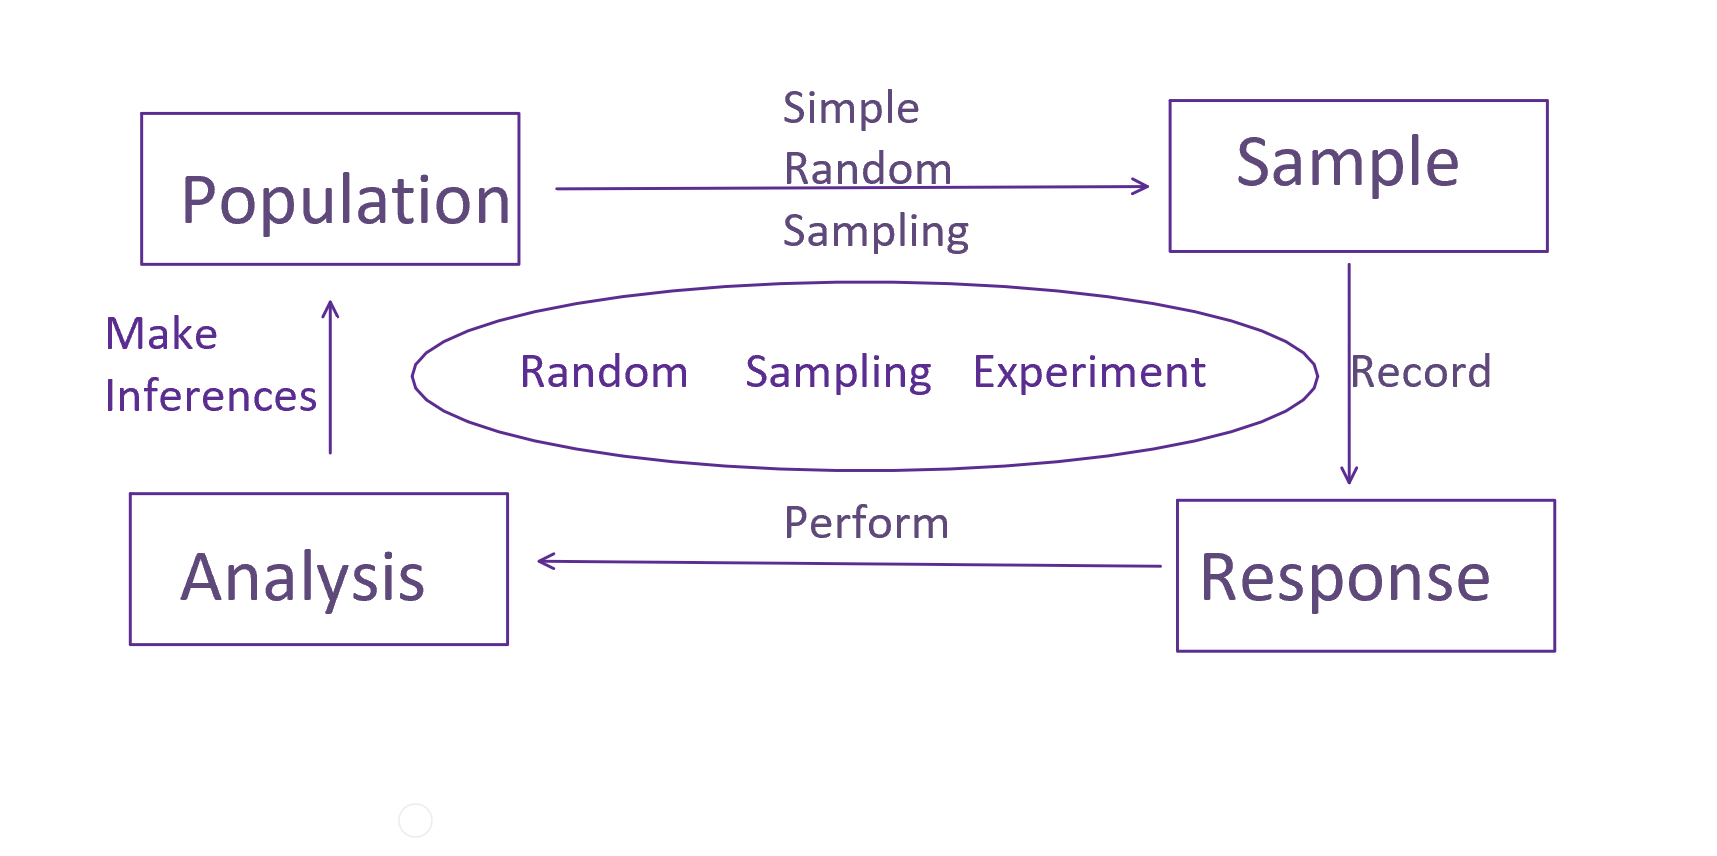
\includegraphics{rsediagram.PNG}
A \emph{random sampling, randomized intervention experiment} consists of obtaining a SRS from a population, randomizing an intervention over those samples, and recording a response variable relating to a research question. This type of experiment is often explained by conceptualizing two (or more) different populations. Suppose the experiment is a clinical trial and the intervention consists of receiving a treatment versus no treatment. Then, we can interpret the randomization step as defining two SRSs from two (abstract or hypothetical) populations: a sample from the set of treated patients and a sample from the set of untreated patients. The research question typically concerns the relationship between these two populations, such as, ``are treated patients, on average, healthier than untreated patients, with respect to the response variable?''

We will only consider randomized interventional experiments. Briefly, consider what can go wrong if we do not randomize intervention. Suppose the patients in our clinical trial consist of both old and young people and that old people are generally more in need of treatment. If we give the treatment to only young(old) people, then we will underestimate(overestimate) the effect of the treatment compared to what its effect would be, on average, over the whole population. In effect, we have \emph{confounded} the treatment/intervention effect with the effect of age on the response. This may seem like a silly example because we could easily avoid assigning the intervention to only young or only old people. But, not all potential confounding variables are obvious/visible. Unknown confounders, also called \emph{lurking variables}, can only be systematically accounted for via randomizing the intervention. Of course it is possible for randomized groups not to be representative in a particular occurrence, but, systematically, randomized groups will tend to be representative, so it's a good practice.

When the intervention is randomized we cautiously assume substantial differences in the observed responses between intervention groups can be attributed to the intervention. In other words, we believe in \emph{causation}---that the intervention caused the observed differences. When confounding variables are present we never know which variable is responsible for observed differences in responses and we cannot support claims about cause and effect relationships using the data alone.

In some studies researchers analyze the relationships between variables without performing randomized interventions; these are usually \emph{observational studies}. For instance, in the Framingham Heart Study, researchers recorded the health and lifestyle choices of Massachusetts residents over several years. By collecting a large amount of data they were able to establish a strong relationship or \emph{association} between cigarette smoking and cancer. Their data alone is not enough to imply causation, but their study inspired many follow-up experiments like lab experiments on animals, and the development of biochemical theories about tumor development. The combination of these various works leaves little doubt today that tobacco use dramatically increases the likelihood of developing cancer.

\hypertarget{the-role-of-probability}{%
\section{The role of probability}\label{the-role-of-probability}}

Consider the example of a political poll on the preferences of voters between two candidates---this is a random sampling experiment. The population consists of all eligible voters in the upcoming election. Each voter can be associated, say, with a 1 or a 0, indicating their preference between the two candidates. Let these 0-1 preferences be denoted \(x_1, \ldots, x_N\) where \(N\) is the population size. There exists a population level value \(\theta\) equal to
\[\theta:=N^{-1}\sum_{j=1}^N x_j\]
denoting the population voter preference; this is the \emph{population proportion}. Most research questions of interest concern the unknown value of \(\theta\). In the polling experiment we observe a random subset of \(x_1, \ldots, x_N\) values, say, \(X_1, \ldots, X_n\) for \(n<N\)---keep in mind these are not the first \(n\) x's, but a random subset of \(n\) x's. Correspondingly, we can compute the sample voter preference
\[\hat\theta_n := n^{-1}\sum_{i=1}^n X_i.\]
For every possible sample of \(n\) voters, there is a corresponding value of \(\hat\theta_n\). We can think of the polling experiment as randomly choosing one of these \(\hat\theta_n\) values out of a hat containing all of them. Randomly sampling voters causes randomness in the observed \(\hat\theta_n\) preference value. The mathematics of \emph{probability} is used to quantify this randomness, e.g., to be able to compute the chance of \(\hat\theta_n\) taking on any particular value, given knowledge of the population.

That last phrase ``given knowledge of the population'' is very important, and illustrates the difference between probability and statistics (inference) quite succinctly. Probability characterizes the chance of observing a particular random sample given the population, whereas statistics seeks to explain some characteristic of the unknown/unobserved population given only one sample (subset of population individuals).

Probability plays a key role in statistics problems, and the first part of our course is devoted to developing methods for computing probabilities of samples in a variety of useful special cases.

Let's illustrate this interplay of probability and statistics by continuing the example of a poll. The population, again, can be represented by \(N\) values, each either a \(0\) or a \(1\) indicating each voter's preferences, and we can label these \(x_1, \ldots, x_N\). A poll is a random sample of \(n\) of these values, labeled \(X_1, \ldots,X_n\), without replacement, i.e., once a value \(x_j\) is selected and recorded it cannot be selected again (no double voting!). The population preference \(\theta\) is the average of \(x_j\)'s for \(j=1, \ldots, N\). If we knew the size of the population \(N\) and the population proportion \(\theta\), then we could compute the chance of observing any \(\hat\theta_n := n^{-1}\sum_{i=1}^n X_i\) value according to the rules of probability (which we will soon study). For example, if \(N\) is much larger than \(n = 10\) and \(\theta = 1/2\), then the chance of observing exactly \(\hat\theta = 1/2\) is about \(25\%\) (it's about equal to \(252\theta^5(1-\theta)^5\)). Of course, the whole point of the poll is to learn something about the unknown value of \(\theta\), so we cannot actually perform this probability calculation in practice. But, consider connecting the probability calculation to our goal. We would like to distinguish between values of \(\theta\) that are more or less plausible. Suppose we conduct the poll of \(10\) individuals and observe \(\hat\theta = 1/2\). Then, our probability calculation says the probability we observe \(\hat\theta = 1/2\) is highest if \(\theta = 1/2\). In other words, \(1/2\) is the most plausible value of the population proportion given our observations. Intuitively, we expect values near \(1/2\) are more plausible than values far from \(1/2\). This correspondence between the probability calculation and plausible values of the \emph{population parameter} is called the \emph{maximum likelihood principle} which we will study in a later chapter.

\hypertarget{exercises}{%
\section{Exercises}\label{exercises}}

\begin{enumerate}
\def\labelenumi{\arabic{enumi}.}
\item
  Google James Lind's Scurvy experiments. What was James' research question? What was the population? Did he obtain a random sample from the population? If not, does that make you suspicious of his findings? Why or why not? Did James use any interventions? If so did he randomize them? Do you think his randomization scheme is reliable? What were his conclusions?
\item
  Find a recent example of an experiment in the news or a scientific publication. Describe the research question, population, intervention (if there is one), and response. Is it a random sampling experiment, a random sample randomized intervention experiment, or something else, like an observational study?
\item
  The Challenger space shuttle exploded when it experienced o-ring failures thought to be caused by low launch temperature. The launch temperature was 31 degrees Fahrenheit. The following data can be interpreted as a random sample of counts of o-ring failures from a population of launches. Given this data do you think we can make reliable conclusions about launch safety at 31 degrees launch temperature? What concepts discussed in this section are relevant here?
\end{enumerate}

\begin{table}

\caption{\label{tab:unnamed-chunk-2}A table of o rings at risk, o ring failires, and launch temperatures of space shuttle flights.}
\centering
\begin{tabular}[t]{rrr}
\toprule
at risk & failed & launch temp.\\
\midrule
6 & 1 & 70\\
6 & 0 & 69\\
6 & 0 & 68\\
6 & 0 & 67\\
6 & 0 & 72\\
\addlinespace
6 & 0 & 73\\
6 & 0 & 70\\
6 & 1 & 57\\
6 & 1 & 63\\
6 & 1 & 70\\
\addlinespace
6 & 0 & 78\\
6 & 0 & 67\\
6 & 2 & 53\\
6 & 0 & 67\\
6 & 0 & 75\\
\addlinespace
6 & 0 & 70\\
6 & 0 & 81\\
6 & 0 & 76\\
6 & 0 & 79\\
6 & 0 & 75\\
\addlinespace
6 & 0 & 76\\
6 & 1 & 58\\
\bottomrule
\end{tabular}
\end{table}

\hypertarget{probability-and-counting}{%
\chapter{Probability and Counting}\label{probability-and-counting}}

Probability is a tricky subject. We have an intuitive sense about probability, but we use it in different ways, which can sometimes lead to confusion. Probability is used in at least two ways:
-to describe the relative frequency of events, e.g., what is the chance of observing 5 heads in the next ten flips of a fair coin; and,
-to communicate degrees of belief, e.g., the Packers have a 30\% chance of winning the Super Bowl.

We will use probability exclusively in the sense of the first interpretation---to characterize the chances of different outcomes in repeatable trials. This sense of probability corresponds to characterizing the possible outcomes of random sampling. Although probability is often used to communicate degrees of belief there are good reasons not to use it for this purpose, but a formal, nuanced discussion of quantification of beliefs is outside our present purview.

\hypertarget{terminology}{%
\section{Terminology}\label{terminology}}

In our discussion of probability we will think of an \emph{experiment} as the act of measuring/observing a variable on one or more random samples from a population. The \emph{sample space} is the set of possible realizations of the experiment. For example, if the experiment is to flip one coin and record whether it is heads or tails, then we can think of this as a random sampling from sample space \(\{H, T\}\) where the outcome may be either \(\{H\}\) or \(\{T\}\). Any subset of the sample space of an experiment is an \emph{event}; for example, \(\{H\}\) and \(\{H,T\}\) are events, and so is \(\emptyset\) which denotes the ``empty set'', the set of nothing.

\hypertarget{set-relations}{%
\section{Set relations}\label{set-relations}}

Events and sample spaces are sets, and we will make use of relations between sets.
-Set union: for sets/events A and B, \(A\cup B\) denotes the set of elements in at least one of \(A\) or \(B\). For example, \(\{1,2,3\}\cup\{3,4,5\} = \{1,2,3,4,5\}\).
-Set intersection: \(A\cap B\) denotes the set of elements in both A and B. For example, \(\{1,2,3\}\cap\{3,4,5\} = \{3\}\).
-Set complement: \(A^c\) denotes the set of elements in the sample space \(\mathcal{S}\) but not in \(A\). For example, if \(\mathcal{S} = \{1,2,3,4,5\}\) then \(A^c = \{4,5\}\).
-Set subtraction: \(A\backslash B\) of \(A-B\) means \(A\cap B^c\) which is the set of elements in \(A\) but not in \(B\). For example, \(\{1,2,3\}-\{3,4,5\} = \{1,2\}\).\\

\hypertarget{sample-space-example}{%
\subsection{Sample space example}\label{sample-space-example}}

Here's an example to illustrate sample spaces. A gas station has six pumps, A, B, C, D, E, F.
-What is the sample space of the number of pumps in use? \(\mathcal{S} =\{0,1,2,3,4,5,6\}\).
-What is the sample space of pumps in use? \(\mathcal{S} = \{\{A,B,C,D,E,F\},\{A,B,C,D,E\}, \ldots,\{F\}, \emptyset \}\). This is the \emph{power set} of \(\{A,B,C,D,E,F\}\), the set of all subsets of those pumps. Fun fact: if the sample space \(\mathcal{S}\) consists of \(N\) elements then its power set, written \(2^{\mathcal{S}}\), contains \(2^N\) elements. Can you see why?
-Suppose you test pump A every day until it fails to function. What is the sample space of this experiment? \(\mathcal{S} = \{F, SF, SSF, \ldots \}\). This is a \emph{countably infinite} sample space.
-You measure the amount of gas pumped by the next customer. \(\mathcal{S} = (0, ?)\), an interval with some upper bound equal to however much gas the station has available. This is an \emph{uncountably infinite} sample space.

\hypertarget{set-relations-example}{%
\subsection{Set relations example}\label{set-relations-example}}

This next example illustrates set relations.\\
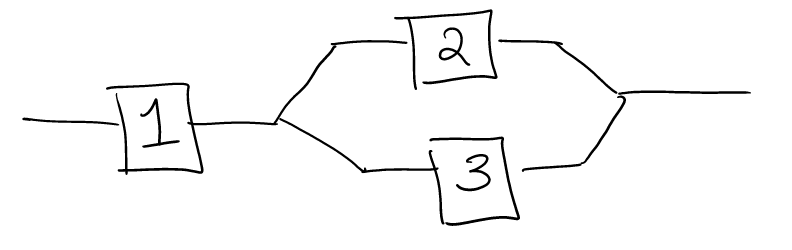
\includegraphics{system.PNG}
Consider this system of series and parallel components. Each component either functions/succeeds (S) or fails (F). The experiment simply observes if the system functions/succeeds or fails.
-What is the sample space in terms of the three components? \(\mathcal{S} = \{SSS, SSF, SFS, FSS, SFF, FFS, FSF, FFF\}\).
-Find the even two components succeed. \(A = \{SSF, SFS, FSS\}\).
-Find the even at leas two components succeed. \(B = \{SSF, SFS, FSS, SSS\} = A\cup \{SSS\}\).
-Find the event the system functions. \(C = \{SSS, SFS, SSF\}\).

\hypertarget{probability-axioms}{%
\section{Probability Axioms}\label{probability-axioms}}

Andrey Kolmogorov formalized rules/axioms of probability we are mostly, intuitively familiar with.

\begin{enumerate}
\def\labelenumi{\arabic{enumi}.}
\tightlist
\item
  The probability of the sample space is 1, \(P(\mathcal{S})=1\).
\item
  Probabilities are non-negative. If \(A\subset\mathcal{S}\) then \(P(A)\geq 0\).
\item
  Countable additivity. This last one is a bit tricky. Let's start with an intuitive, simpler case. Suppose \(\mathcal{S} = \{1,2,3,4,5\}\). The important part is \(\mathcal{S}\) is finite and includes only different things that don't ``overlap''. Then, we know that, for example, \(P(\{1\}\cup \{2\}) = P(\{1\}) + P(\{2\})\), which says that the probability of the union of \emph{disjoint} events equals the sum of probabilities of each event. Kolmogorov requires this extends to countably infinite \(\mathcal{S}\), hence the name countable additivity. Specifically, let events \(A_1\), \(A_2\), \(\ldots\) be a sequence of mutually disjoint events (none overlap, like pizza slices) so that \(A_i \cap A_j = \emptyset\) for every \(i\ne j\). Then,
  \[P\left(\bigcup_{i=1}^\infty A_i\right) = \sum_{i=1}^\infty P(A_i).\]
\end{enumerate}

There are a number of important consequences of the axioms:
* Complementarity - \(P(A^c) = 1-P(A)\)
* Inclusion-exclusion principle
\[P(A\cup B) = P(\{A\cap B\}\cup\{A-B\}\cup\{B-A\})\]
\[ = P(A)+P(B)-P(A\cap B)\]

\hypertarget{example-of-using-the-probability-axioms}{%
\subsection{Example of using the probability axioms}\label{example-of-using-the-probability-axioms}}

Suppose we are inspecting a product for defects. Three types of defects are possible. Let \(A_j\), \(j=1, 2, 3\) denote the events that a defect of type \(j\) is present. We are given \(P(A_1) = 12\%\), \(P(A_2) = 7\%\), \(P(A_3) = 5\%\), \(P(A_1\cup A_2) = 13\%\), \(P(A_1 \cup A_3) = 14\%\), \(P(A_2 \cup A_3) = 10\%\), and \(P(A_1\cap A_2\cap A_3) = 1\%\).
1. Find \(P(A_1^c)\).
\[ = 1-P(A_1) = 88\%\]
2. Find \(P(A_1\cap A_2)\)
\[ = P(A_1) + P(A_2) - P(A_1\cup A_2) = 6\%\]
3. Find \(P(A_1 \cap A_2 \cap A_3^c)\)
\[ = P(A_1\cap A_2) - P(A_1\cap A_2 \cap A_3)\]
\[ = 6\% - 1\% = 5\%\]
4. Find the probability the system has at most 2 defects.
``At most 2'' means ``Not 3'', so
\[P(\text{at most 2 defects}) = 1 - 1\% = 99\%.\]

\hypertarget{equally-likely-outcomes}{%
\section{Equally likely outcomes}\label{equally-likely-outcomes}}

The axioms of probability lay some ground rules probabilites must follow, but don't say much about how to assign probabilities to events. Next up, we'll see how to determine probabilities of events for finite sample spaces.

The principle of \emph{equally likely outcomes} says that a finite sample space \(\mathcal{S}\) of \(N\) disjoint outcomes or elements has equally likely outcomes if the probability of each outcome is \(1/N\). It's clear that this probability assignment obeys the axioms.

From here we can assign probabilites to events \(A\) in \(\mathcal{S}\) by simply counting how many outcomes are contained in \(A\); that is,
\[P(A) = \frac{N(A)}{N}\]
where \(N(A)\) denotes the number of outcomes in \(\mathcal{S}\) contained in \(A\). Therefore, in the context of equally likely outcomes, counting is very important.

Let's take a moment to consider why equally likely outcomes are an important case. We are studying random sampling experiments, and a SRS is defined by the property that every subset of \(n\) population individuals is equally likely to be chosen. So, there's a direct correspondence between the probability setup we're considering here and random sampling experiments.

\hypertarget{some-counting-rules}{%
\section{Some counting rules}\label{some-counting-rules}}

The \emph{product rule} considers the probability of a complex event that can be decomposed into several independent events. For example, suppose the event is generating a random ``word'' that is five (English) letters long. We can decompose this event into randomly sampling (with replacement) from the alphabet of 26 letters 5 times. Each letter we sample is sampled independently (each letter chosen has no influence on the other choices/random draws). The product rule says the number of ways to generate the word (the number of ways the event can happen) is equal to the product of the numbers of ways each letter can be randomly selected (the number of ways each sub-event can happen). For the word example, that's \(26^5\).

Example: You are remodeling your kitchen and have to buy a new refrigerator, oven, and dishwasher. Four brands make fridges, 3 make ovens, and 5 dishwashers. In how many ways can you select three brands? \(4\times 3\times 5 = 60\).

A \emph{combination} is a rule for counting the number of subsets of \(k\) outcomes/items that can be selected from a larger set of \(n\) distinct items. There are \(\frac{n!}{k!(n-k)!}\) also written \({n \choose k}\) such selections.

A \emph{permutation} is similar; it's the number of ways one can select \(k\) distinct items from \(n\) in a particular order. This is \(\frac{n!}{k!}\).

Example: Suppose you win 3 tickets to an NFL playoff game (I wish!). You will choose 2 out of 4 of your closest friends to go with you. How many different choices can you make? It's \({4\choose 2} = \frac{4*3*2*1}{(2*1)(2*1) } = 6\) choices.

Example: In ranked-choice voting you rank your choices by order of preference rather than by voting for only one option. If there are ten options, then how many top four rankings are possible? In this case, it's \(\frac{10!}{4!}\) because we consider different orderings to be distinct, of course.

Next we consider a rule for \emph{counting objects of different types}. Suppose we have \(n\) objects: \(n_1\) of type 1, \(n_2\) of type 2, \ldots{} and \(n_k\) of type \(k\) such that \(n=\sum_{j=1}^k n_j\). Items of the same type are indistinguishable. The number of distinct/distinguishable arrangements of the \(n\) objects is \(\frac{n!}{n_1!\times n_2! \times \cdots \times n_k! }\).

For example, if we file a 6-sided die 20 times and obtain 6 ones 3 twos 4 threes and 7 fours the number of distinct orderings of those outcomes is \(\frac{20!}{6!3!4!7!}\).

\hypertarget{applications-to-random-sampling}{%
\section{Applications to random sampling}\label{applications-to-random-sampling}}

Consider flipping a fair coin \(20\) times. This can be thought of as an event decomposed into 20 independent sub-events---the different flips. The product rule says there are \(N = 2^{20}\) possible outcomes. Next, consider how many outcomes have \(5\) heads. This is the number of distinct arrangements of 5 heads and 15 tails, which equals \(\frac{20!}{5!15!}\). Putting these together, the probability of exactly 5 heads in 20 flips is
\[\frac{20!}{5!15!}(\frac{1}{2})^{20}.\]
We can generalize this to \(n\) flips and \(x\) heads, easily enough\ldots{} The probability of \(x\) heads in \(n\) flips is
\[P(x) = \frac{n!}{x!(n-x)!}(\frac{1}{2})^n.\]

This coin-flipping experiment is an example of random sampling with replacement. Each flip is a random draw from a population of \(2\) coins in which \(1\) is heads and \(1\) is tails. Each coin is equally likely to be chosen. And, once selected and recorded, the coin is then returned. Alternatively, we could imagine the experiment as random sampling without replacement from an infinite population of coins for which ``half'' are heads.

For a more concrete example of sampling without replacement, consider the following. Suppose the statistics department has 15 microsoft and 10 mac laptops available for lending, and suppose 6 are chosen as a SRS. What is the probability 3 of the chosen laptops are microsoft and the other 3 mac? There are \(N = {25 \choose 6}\) ways to select 6 at random. There are \({15 \choose 3}\) ways to select 3 microsoft and \({10 \choose 3}\) ways to select \(3\) mac laptops. Therefore, the probability is the ratio
\[\frac{{15 \choose 3}\times {10 \choose 3}}{{25 \choose 6}}.\]

\hypertarget{exercises-1}{%
\section{Exercises}\label{exercises-1}}

\begin{enumerate}
\def\labelenumi{\arabic{enumi}.}
\tightlist
\item
  An Amazon warehouse employs twenty workers on early shift, 15 on the late shift, and 10 on the overnight shift. Six workers are randomly selected (without replacement) fora safety interview.
\end{enumerate}

\begin{enumerate}
\def\labelenumi{\alph{enumi}.}
\tightlist
\item
  How many selections result in 6 workers from the early shift? What is the probability of this event?
\item
  What is the probability all 6 workers selected come from the same shift?
\item
  What is the probability at least two different shifts are represented among the six workers selected?
\item
  What is the probability at least one shift is not represented?
\end{enumerate}

Answers:
a. \({20 \choose 6}\), and \(\frac{{20 \choose 6}}{{45 \choose 6}}\)
b. \(\frac{{20 \choose 6}+{15 \choose 6}+{10 \choose 6}}{{45 \choose 6}}\)
c.~\(1-\)the probability in b.
d.~\(\frac{{35 \choose 6}+{30 \choose 6}+{25 \choose 6}}{{45 \choose 6}}\)

\begin{enumerate}
\def\labelenumi{\arabic{enumi}.}
\setcounter{enumi}{1}
\tightlist
\item
  Suppose a chain molecule consists of 3 sub-molecules of type A, 3 of B, 3 of C, and 3 of D, e.g., ABCDABCDABCD.\\
\end{enumerate}

\begin{enumerate}
\def\labelenumi{\alph{enumi}.}
\tightlist
\item
  How many such distinguishable chain molecules are there of any order?
\item
  If we randomly selected a chain molecule, what tis the probability that all three sub-molecules of each type are ``lined up'', e.g., BBBAAADDDCCC?
\end{enumerate}

Answers:
a. \(\frac{12!}{(3!)^4}\)
b. \(\frac{4!(3!)^4}{12!}\)
3. A quality control inspector must examine a part from each of 4 different bins. The bins contain 5, 2, 6, and 3 parts, respectively. In how many different ways can the inspector choose the 4 parts?

\begin{enumerate}
\def\labelenumi{\arabic{enumi}.}
\setcounter{enumi}{3}
\tightlist
\item
  In order to meet the requirements of a new housing code, each apartment complex in a certain neighborhood must have the smoke detectors from 3 apartments checked by the fire chief each year. In how many ways can the fire chief choose 3 apartments from a complex containing 20 apartments?
\end{enumerate}

\begin{enumerate}
\def\labelenumi{\arabic{enumi}.}
\setcounter{enumi}{4}
\tightlist
\item
  A ten person City Council must elect a Chair, a Vice Chair, and a Secretary. In how many ways can the positions be filled?
\end{enumerate}

\begin{enumerate}
\def\labelenumi{\arabic{enumi}.}
\setcounter{enumi}{5}
\tightlist
\item
  The driving route you use to travel to and from work and your home includes two stop lights. Let \(A\) and \(B\) denote the events you stop and the first light and the second light, respectively. Suppose \(P(A) = 0.4\), \(P(B) = 0.5\), and \(P(A\cup B) = 0.6\). Find:
\end{enumerate}

\begin{enumerate}
\def\labelenumi{\alph{enumi}.}
\tightlist
\item
  \(P(A\cap B)\), the probability you stop at both lights
\item
  \(P(A \cap B^c)\), the probability you stop at only the first light
\item
  \(P(B \cap A^c)\), the probability you stop at only the second light
\end{enumerate}

\hypertarget{conditional-probabilities-of-events}{%
\chapter{Conditional probabilities of events}\label{conditional-probabilities-of-events}}

Let \(A\) and \(B\) denote events in a sample space \(\mathcal{S}\). Suppose we know \(B\) occurs. Then, \(P(A|B)\) denotes the \textbf{conditional probability} of \(A\) given \(B\). This has the mathematical formula
\[P(A|B) = \frac{P(A\cap B)}{P(B)}.\]
In this formula, \(B\) acts as the new or conditional sample space. It is always true
\[P(A|\mathcal{S}) = \frac{P(A\cap \mathcal{S})}{P(\mathcal{S})} = \frac{P(A)}{1} = P(A).\]
Knowing \(B\) happens is equivalent to changing the sample space to \(B\).

\hypertarget{example}{%
\subsection{Example}\label{example}}

Four individuals are donating blood to a blood bank. Their blood types are unknown. If exactly 1 of them is O+, then what is the probability at least 3 are typed in order to obtain an O+ sample?
Answer:
\[P(\text{at least three must be typed}) = P(3) + P(4).\]
\[P(3) = P(\text{first is not O+ and second is not O+ and third is O+}).\]
\[ = P(\text{first is not O+})P(\text{second is not O+ given first is not O+})P(\text{third is O+ given first two are not})\]
\[ = \frac{3}{4}\times \frac{2}{3}\times \frac{1}{2}.\]
We used a (perhaps intuitive) extension of the conditional probability formula above:
\[P(A\cap B\cap C) = P(C|A\cap B)P(A \cap B) = P(C|A\cap B)P(B|A)P(A)\]
Here, \(A\), \(B\), and \(C\) represent the first, second, and third blood typings.

\hypertarget{example-1}{%
\subsection{Example}\label{example-1}}

Let \(A\) be the event a randomly selected adult male US citizen is at least 6'3'' tall. Let \(B\) be the event a randomly selected adult male US citizen is an NBA player. Which is larger, \(P(A|B)\) or \(P(B|A)\)?

Answer:
Be careful; these can be tricky. \(P(A)\) is much larger than \(P(B)\) because there are many more male US citizens 6'3'' or taller than there are NBA players (some also may not be US citizens). And, \(P(A|B)\) is much larger than \(P(B|A)\). The reason is that if we condition on US citizen NBA players, almost all of them are 6'3'' or taller. However, if we condition on US males 6'3'' or taller, NBA players are still a tiny proportion.

\hypertarget{example-2}{%
\subsection{Example}\label{example-2}}

Bertrand's Boxes --- There are three boxes: the first has two gold coins, the second one gold and one silver, and the third two silver coins. You choose a box at random and a coin from the box at random. Given you choose a gold coin, what is the probability the other coin in that box is gold?

Answer:

Let \(G_1\) be the event the first coin chosen is gold and let \(G_2\) be the event the second coin chosen (same box) is gold. Let \(B_1\), \(B_2\), and \(B_3\) denote events corresponding to choosing boxes 1, 2, and 3. Then, we seek
\[P(G_2|G_1) = \frac{P(G_1\cap G_2)}{P(G_1)}.\]
\[P(G_1) = P(G_1 \cap B_1) + P(G_1 \cap B_2) + P(G_1 \cap B_3)\]
\[ = P(G_1 | B_1)P(B_1) + P(G_1 | B_2)P(B_2)+ P(G_1 | B_3)P(B_3)\]
\[ = 1 \times 1/3 + 1/2 \times 1/3 + 0 \times 1 /3 = 1/2.\]
\[P(G_1\cap G_2) = P(\text{chose box 1}) = P(B_1) = 1/3.\]
Therefore,
\[P(G_2|G_1) = \frac{1/3}{1/2} = 2/3.\]

Note: This question, which is often called ``Bertrand's Paradox'', has caused an awful lot of consternation and controversy. When pondering this question for the first time, many people will (incorrectly) suppose the answer is 1/2. Their logic is that since the first coin was gold, then either the first or second box was chosen. Then, those boxes being equally likely, there is a 1/2 chance box 1 was chosen, and, therefore, the chance of the second coin being gold is 1/2. The first part of that logic is well-founded: the third box could not have been chosen. However, the fact the first coin is gold also implies we were more likely to have chosen the first box than the second---those two boxes are not equally likely in light of the information that the first coin was gold. Indeed, we could have simply asked ``what is the chance we selected box 1 given the coin is gold?''---that question is equivalent to asking the chance the second coin is gold. When rephrased this way, most people find it easier to see that the chosen box is more likely box 1 than box 2 (twice as likely, in particular), given the first coin selected is gold.

\hypertarget{bayes-rule}{%
\section{Bayes' rule}\label{bayes-rule}}

In the example of Bertrand's Paradox you might have noticed we used a slick trick to compute \(P(G_1)\)---we \textbf{partitioned} the event \(G_1\) into three pieces \(G_1 = \{G_1 \cap B_1\}\cup \{G_1 \cap B_2\}\cup \{G_1 \cap B_3\}\) where \(\{B_1 \cup B_2 \cup B_3\} = \mathcal{S}\). Partitioning is the act of subdividing a set into non-overlapping, or \textbf{disjoint}, subsets. This way, we can represent a set as a union of subsets, much like a pizza is equivalent to the collection of pizza slices. This partitioning trick is useful enough to be given a name, \emph{the Law of Total Probability}: If \(A_1, \ldots, A_n\) is a collection of disjoint subsets of \(\mathcal{S}\) such that \(\mathcal{S} = \bigcup_{i=1}^n A_i\) (i.e., the collection is exhaustive), then for any \(B\subset \mathcal{S}\)
\[P(B) = \sum_{i=1}^n P(B \cap A_i) = \sum_{i=1}^n P(B | A_i)P(A_i).\]
Recall the axiom of countable additivity; it's basically equivalent to the law of total probability.

Often times information is known about certain conditional probabilities---\(P(A|B)\)---but we want to know the reverse conditional probability \(P(B|A)\). Bayes' rule provides a formula for computing these reverse conditional probabilities. There's not really anything special about the formula; after all, it follows immediately from the definition of conditional probability:
\[P(A|B) = \frac{P(A\cap B)}{P(B)} = \frac{P(A\cap B)P(A)}{P(B)P(A)} = \frac{P(B|A)P(A)}{P(B)}.\]
Or, in other words,
\[P(A|B)P(B) = P(B|A)P(A).\]

\hypertarget{example-3}{%
\subsection{Example}\label{example-3}}

Perhaps the most famous example of Bayes' rule illustrates the difficulty in detecting rare events. Suppose 1 in 1000 adults suffers from a (fairly rare) disease. A diagnostic test is 99\% effective in detecting disease among individuals who have the disease. Among people who do not have the disease, the diagnostic test is nevertheless positive 2\% of the time. Given the test is positive, what is the chance the individual tested has the disease?

Answer:
Let \(A\) be the event the test is positive and let \(B\) be the event the individual tested has the disease. Then, we are given \(P(B) = 0.001\). By the law of total probablity
\[P(A) = P(A\cap B)+P(A\cap B^c) = P(A| B)P(B)+P(A| B^c)P(B^c) = 0.99\times 0.001 + 0.02\times 0.999 = 0.02097\]
We want to find \(P(B|A)\), which is equal to \(P(A|B)P(B)/P(A)\) by Bayes' rule. So,
\[P(B|A) = P(A|B)P(B)/P(A) = 0.99\times 0.001 / 0.02097 = 0.0472103.\]
This is a terrible diagnostic test. Less than 5\% of people who test positive actually have the disease.

\hypertarget{independence}{%
\section{Independence}\label{independence}}

Two events \(A\) and \(B\) are independent if
\[P(A|B) = P(A).\]
In other words, knowing \(B\) happens does not affect the chance of \(A\) happening. By using the definition of conditional probablity, it follows that
\[P(A|B) = \frac{P(A\cap B)}{P(B)} \stackrel{ind.}{=}P(A)\Rightarrow P(A\cap B) = P(A)P(B).\]
Further, if \(P(A\cap B) = P(A)P(B)\) then, again using the definition of conditional probability
\[P(A|B) = \frac{P(A\cap B)}{P(B)} = \frac{P(A)P(B)}{P(B)} = P(A).\]
Therefore, independence of two events \(A\) and \(B\) is equivalent to the \emph{product rule} being satisfied:
\[A\text{ and }B\text{ independent } \iff P(A\cap B) = P(A)P(B).\]

Independence extends to collections of events. For example, intuitively we know two rolls of a die are independent. But, ther'e nothing special about rolling a die twice; three or more rolls are also, intuitively, mutually independent. To be precise, we say a collection of events \(A_1, A_2, \ldots\) is \emph{pairwise independent} if for every pair \(A_i, A_j\), \(i\ne j\) the product rule holds: \(P(A_i \cap A_j) = P(A_i)P(A_j)\). Furthermore, a collection of events \(A_1, A_2, \ldots\) with index set equal to the natural numbers \(\mathbb{N}\) (or a finite subset) is \emph{mutually independent} if every subset \(\{A_i, i\in I, I\subset \mathbb{N}\}\) of events obeys the product rule: \(P( \bigcap_{i \in I} A_i) = \prod_{i \in I} P(A_i)\).

Example: Consider rolling a fair die \(n\) times and recording the outcomes. Let \(A_i,\) \(i = 1,\ldots,n\) be the event the \(i^{th}\) roll is odd. The set \(\{A_i, i=1, \ldots, n\}\) is mutually independent.

Example: Let \(A\) and \(B\) denote the events that the first and second tosses of a fair coin are heads. These are independent events. Define \(C = \{\{A\cup B\}-\{A\cap B\}\}\). Then, \(A\) and \(C\) are pairwise independent. To see this, compute:
\[P(A \cap C) = P(A \cap \{\{A \cap B^c\} \cup \{A^c \cap  B\}\}) = P(A \cap \{A \cap B^c\}) + P(A \cap \{A^c \cap  B\}) = P(A \cap B^c) = P(A)(1-P(B)) = 0.25\]
\[P(C) = P(A \cap B^c) + P(A^c \cap B) = P(A) - P(A)P(B) + P(B)- P(A)P(B) = 0.5\]
\[P(A)P(C) = 0.25\]
But, A, B, and C are not mutually independent because
\[\{A\cap B\cap C\} = \{\{A\cap B\}\cap \{A \cap B^c\}\} \cup \{\{A\cap B\}\cap \{A^c \cap B\}\} = \emptyset\]
So, \(P(A\cap B\cap C) = 0\), while \(P(A)P(B)P(C) = 0.125\).

\hypertarget{exercises-2}{%
\section{Exercises}\label{exercises-2}}

\begin{enumerate}
\def\labelenumi{\arabic{enumi}.}
\tightlist
\item
  Seventy percent of small, private-use aircraft that disappear in flight are eventually discovered. Of the aircraft that are discovered, \(60\%\) have a black box, whereas \(90\%\) of the missing aircraft that are not discovered do not have a black box. Suppose an aircraft has disappeared.
\end{enumerate}

\begin{enumerate}
\def\labelenumi{\alph{enumi}.}
\tightlist
\item
  If it has a black box what is the probability it will not be discovered?
\item
  If it does not have a black box what is the probability it will be discovered?
\end{enumerate}

\begin{enumerate}
\def\labelenumi{\arabic{enumi}.}
\setcounter{enumi}{1}
\tightlist
\item
  Consider rolling two different fair, six-sided dice, one red and one green. Let \(A\) be the event the red die is 3, \(B\) be the event the green die is \(4\), and \(C\) be the event the sum of the two die is \(7\).
\end{enumerate}

\begin{enumerate}
\def\labelenumi{\alph{enumi}.}
\tightlist
\item
  Are \(A\) and \(B\) independent?
\item
  Are \(B\) and \(C\) independent?
\item
  Are \(A\) and \(C\) independent?
\item
  Are the three events mutually independent?
\end{enumerate}

\hypertarget{random-variables}{%
\chapter{Random Variables}\label{random-variables}}

\hypertarget{random-variables-1}{%
\section{Random variables}\label{random-variables-1}}

So far, we've discussed probabilities for events that are subsets of simple, finite sample spaces. However, often we are interested in continuous measurements/responses on sampled individuals, so we need to expand our probability calculus to accomodate this more general situation.

Let \(X\) denote a numerical response or function of a random sample from \(\mathcal{S}\). For a basic example, consider the experiment of flipping a fair coin and recording the outcome. Then \(\mathcal{S} = \{H, T\}\), but we might map heads and tails to the numbers 1 and 0. Therefore, let \(X:\{H,T\}\mapsto \{1,0\}\) with \(X(H) = 1\) and \(X(T) = 0\) denote this mapping/function. \(X\) is a \emph{random variable}---or mapping---defined on the space \(\{0,1\}\), taking the sample space as domain and some space of numbers as its codomain.

In many cases we will consider \emph{continuous random variables}, mappings with codomain equal to the real numbers, denoted \(\mathbb{R}\), or some (uncountable) subset thereof, like the interval \((0,1)\).

In contrast, when the codomain of a random variable is a countable set of numbers, e.g., the positive integers, then we call it a \emph{discrete random variable}.

\hypertarget{examples-of-discrete-r.v.s}{%
\subsection{Examples of Discrete r.v.'s}\label{examples-of-discrete-r.v.s}}

\begin{enumerate}
\def\labelenumi{\arabic{enumi}.}
\item
  Consider an experiment in ehich a mechanical dialer machine randomly dials phone numbers with a given area code. This is a common practice in polling. Let \(Y\) denote the random variable with value \(1\) if the dialed number is on a ``do not call list'' and zero otherwise. A random variable (r.v.) that can only take values 0 or 1 is called a Bernoulli random variable. (Oddly enough, a random variable that can only take values 1 or -1 is called a Rademacher r.v. !)
\item
  A quality control test is used to test the strength of concrete beams. The test exposes beams to both shear forces and flexure forces until each beam fails. An experiment randomly selects three failed beams and observes whether each failed due to shear (S) or flexure (F) forces. The sample space is:
  \[\mathcal{S} = \{SSS, SSF, SFS, FSS, SFF, FFS, FSF, FFF\}.\]
  Let \(X\) denote the random variable that counts the number of beams that fail due to flexure force. It has codomain \(\{0,1,2,3\}\) and is defined by the mapping
  \[X(SSS) = 3, \, X(SSF) = 1, \, \ldots, X(FFF) = 0.\]
\item
  In the context of 2. above suppose an experiment randomly selects a failed beam and measures the force \(X\) applied at point of failure in Newtons. Consider the sample space of all hypothetical concrete beams that could be tested. Then, \(X\) is a continuous r.v. with codomain \((0,U)\) for some upper bound \(U\). Depending on what is known about the beams, we may take \(U\) to be a specified upper bound, or we may set \(U = \infty\). More on this later\ldots{}
\end{enumerate}

\hypertarget{probability-mass-functions}{%
\section{Probability Mass Functions}\label{probability-mass-functions}}

A \emph{probability mass function} or PMF is a function that assigns probabilities to values of discrete r.v.'s. We'll write \(p(x)\) for the PMF of a r.v. \(X\) where \(x\) indicates any value in the codomain of \(X\). When \(X\) is a finite r.v. with only a small number of possible values its PMF can be conveniently expressed as a table of values. For example, in the concrete beam example in 2. above we have
\[x: 0 \quad 1\quad 2\quad 3\]
\[p(x):1/8\quad 3/8\quad 3/8 \quad 1/8\]

We can also represent PMFs using a function. For example, the probability \(x\) heads are observed in 20 flips of a fair coins is given by \(p(x) = {20 \choose x}(\frac{1}{2})^{20}\). Find a plot of this PMF below. Notice it is a graph of a discontinuous function, a plot of 21 discrete points or ``masses''. This is how we get the name ``probability mass function''---the probabilities are like discrete ``masses'' when displayed in a plot, in contrast to a smooth continuous function.
\includegraphics{04-Random-Variables_files/figure-latex/unnamed-chunk-1-1.pdf}

Example: Suppose a contractor needs between 1 and 5 (inclusive) permits for a construction job. If \(p(x)\propto x^2\) then find \(p(x)\). The key is that \(\sum_{x=1}^5 p(x) = 1\). Therefore, we need to find the proportionality constant \(C\) satisfying \(C(1^2+2^2+3^2+4^2+5^2) = 1\). Verify \(p(x) = x^2 / 55\).

\hypertarget{cumulative-mass-functions}{%
\section{Cumulative Mass Functions}\label{cumulative-mass-functions}}

A \emph{cumulative mass function} or CMF is a function \(F(t)\) that assigns probabilities to sets of values \(\{x: x\leq t\}\). The CMF is related to the PMF \(p(x)\) in the following way:
\[F(t) = \sum_{x\leq t} p(x).\]

Example: the probability there are at least \(t\) heads in the next \(20\) flips of a fair coin is
\[F(t) = \sum_{x\leq t} {20 \choose t}\left(\frac{1}{2}\right)^{20}\]
where \(t\) can be any non-negative real number. The plot of the CMF is below. Notice it is a step-function. It's smooth and continuous except for the jumps at each integer value. And, notice the heights of the jumps are precisely the PMF values a those jumps.
\includegraphics{04-Random-Variables_files/figure-latex/unnamed-chunk-2-1.pdf}

Example: The CMF in the construciton permits example above may be expressed as follows:
\[F(t) =\left\{ \begin{matrix} 
0  & t < 1 \\ 
1/55 & 1\leq t\leq 2 \\ 
5/55 & 2\leq t\leq 3 \\
14/55 & 3\leq t\leq 4 \\
30/55 & 4\leq t\leq 5 \\
1 & 5\leq t \\
\end{matrix}\right\}   \]

\hypertarget{examples-of-continuous-r.v.s}{%
\section{Examples of Continuous r.v.'s}\label{examples-of-continuous-r.v.s}}

\begin{enumerate}
\def\labelenumi{\arabic{enumi}.}
\item
  Iowa DoT (Department of Transportation) records the locations of car accidents along interstate 80. Suppose these measurements are recorded as the number of feet past the last mile marker. It makes sense to treat these are continuous measurements on an interval \((0,5280)\) feet.
\item
  During a storm you count the number of seconds between flashes of lightning and subsequent sounds of thunder using a stopwatch with precision in hundredths of a second. It makes sense to treat these measurements of time as continuous random variables taking values in a set of positive real numbers.
\end{enumerate}

\hypertarget{probability-assignments-for-continuous-r.v.s}{%
\section{Probability assignments for continuous r.v.'s}\label{probability-assignments-for-continuous-r.v.s}}

Let \(X\) denote a random variable taking values in a (possibly unbounded) interval of real numbers \((a,b)\). We say \(X\) is a continuous r.v. if it has zero probability of being any particular value, i.e., \(P(X=x) = 0\) for all \(x \in (a,b)\) but has non-negative probability of taking a value in a sub-interval, i.e., \(P(x_1 < X <x_2) \geq 0\) for all \(a\leq x_1 < x_2\leq b\).

Example: Uniform probability assignment. Suppose the probability \(X\) belongs to an interval is proportional to the length of the interval. Then, if \(X \in (a,b)\) we have \(P(a \leq X \leq B) = P(\mathcal{S}) = 1 = \frac{b-a}{b-a}\). And, for any \(a\leq x_1 < x_2\leq b\) we have \(P(x_1 < X < x_2) = \frac{x_2 - x_1}{b-a}\). What is the probability \(X = x\) for any \(x \in (a,b)\)? Take the limit:
\[P(X = x) = \lim_{h\rightarrow 0} P(x \leq X \leq x+h) = \lim_{h\rightarrow 0}\frac{x+h - x}{b-a} = \lim_{h\rightarrow 0}\frac{h}{b-a} = 0.\]

The \emph{probability density function} (PDF) denoted \(f(x)\) is used to assign probabilities to intervals of values in the codomain of a continuous random variable. For a continuous r.v. \(X\), \(f(x)\) satisfies, \(f(x)>0\) for all \(x\) in the codomain of \(X\) and
\[P(a\leq X\leq b) = \int_a^b f(x)dx.\]

The \emph{cumulative probability density} CDF (also call distribution function or cumulative distribution function) denoted \(F(x)\) is defined by the following integration of the PDF
\[F(x) = P(X\leq x) = \int_{-\infty}^x f(t)dt.\]

Warning: the PDF \textbf{does not} assign probabilities to singletons \(\{x\}\); \(f(x)\) does not equal \(P(X=x)\). Rather, \(P(X=x) = \int_x^x f(t)dt = 0\).

Example: Suppose the locations of auto accidents along a 200 mile interval of I-80 in Iowa are distributed uniformly. Then, we can regard the location of the next car accident as a continuous r.v. with CDF \(F(x) = x/200\), and PDF \(f(x) = \frac{d}{dx}F(x) = 1/200\). The chance of the next accident occuring between miles 50 and 55 is \(\frac{55-50}{200} = 0.025\). Find plots of this PDF (red) and CDF (blue) below. The red line is at height 1/200. In particular, not these are smooth functions, in contrast to the PMF and CMF functions above. This smoothness versus discreteness motivated the adjectives ``density'' versus ``mass'', which originated in physics literature.

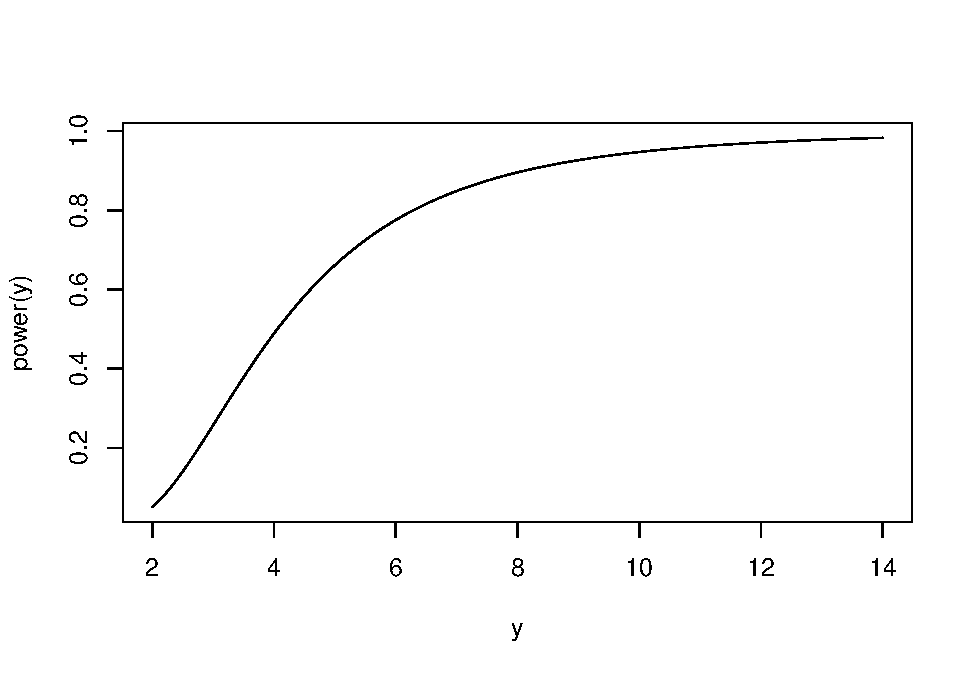
\includegraphics{04-Random-Variables_files/figure-latex/unnamed-chunk-3-1.pdf}

\hypertarget{transformations-of-random-variables}{%
\section{Transformations of random variables}\label{transformations-of-random-variables}}

Let \(X\) denote a continuous random variable with PDF \(f(x)\), and let \(Y = g(X)\) for some function \(g\). What is the probability \(P(Y \leq y)\) for some value \(y = g(x)\)? By definition,
\[F_X(x) = P(X\leq x) = \int_{-\infty}^x f_X(x)dx\]
where \(f_X(x)\) denotes the PDF of \(X\). If \(g\) is invertible, then we can use ``u-substitution'': \(x = g^{-1}(y)\) and \(dx = \frac{1}{g'(x)}dy\) so that
\[F_X(x) = \int_{-\infty}^x f_X(x)dx = \int_{g(-\infty)}^{y=g(x)} \frac{1}{g'(g^{-1}(y))} f_X(g^{-1}(y))dy.\]
And, by differentiating w.r.t. y (and considering the cases \(g\) is increasing versus \(g\) is a decreasing function) we find
\[f_Y(y) = \left|\frac{1}{g'(g^{-1}(y))}\right| f_X(g^{-1}(y)).\]

Example: Let \(X\) be an angle measured in radians selected at random from the interval \([-\pi/2, \pi/2]\) with uniform probability. Then, \(f(x) = \frac{1}{\pi}\) for \(x \in [-\pi/2, \pi/2]\). Let \(Y = \sin X\). The PDF of \(Y\) is given by
\[f_Y(y) = \left|\frac{1}{\sin'(\arcsin y)}\right|\frac{1}{\pi} = \left|\frac{1}{\pi\cos(\arcsin y)}\right| = \frac{1}{\pi(1-y^2)}.\]
The plots below illustrate a random sample of such \(x-\)values along with their transformations to \(y\):

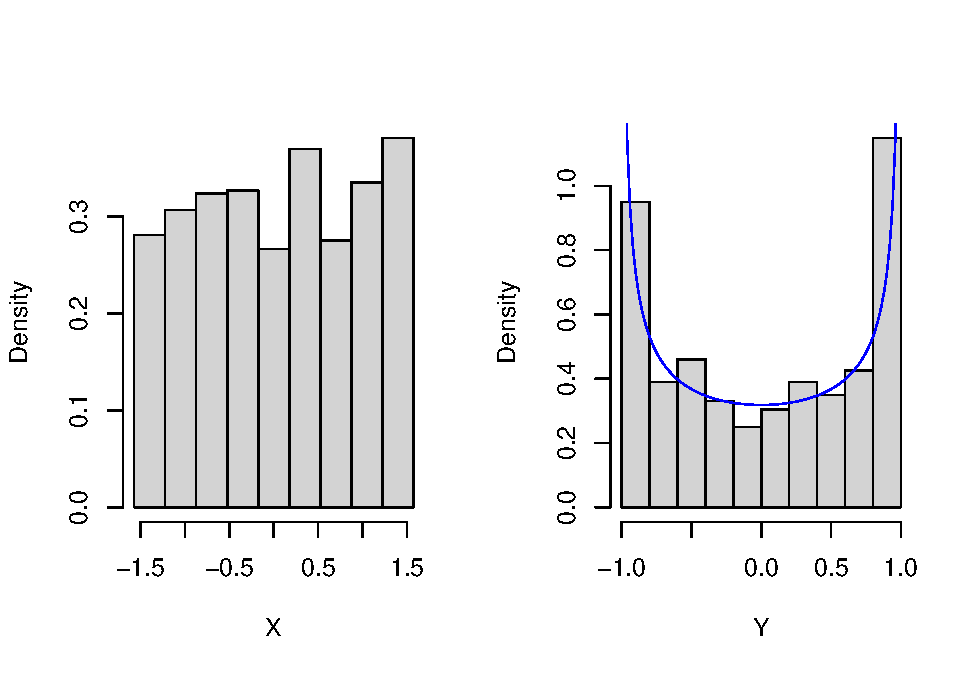
\includegraphics{04-Random-Variables_files/figure-latex/unnamed-chunk-4-1.pdf}

\hypertarget{expectation-of-random-variables}{%
\chapter{Expectation of Random Variables}\label{expectation-of-random-variables}}

\hypertarget{mean-of-a-random-variable}{%
\section{Mean of a Random Variable}\label{mean-of-a-random-variable}}

Let \(X\) be a random variable. Then the \emph{expectation} of \(X\) is denoted \(E(X)\). For discrete \(X\),
\[E(X) = \sum_{x} x p(x)\]
\emph{if it exists\ldots{}} It is possible the sum above diverges, i.e.~equals infinity, in which case we say \(E(X)\) does not exist. For a continuous random variable on \((a,b)\),
\(E(X) = \int_a^b x f(x)dx\). Again, it is possible this integral does not exists, in which case neither does the expectation exists.

Typical notation for \(E(X)\) is \(\mu'\) ``mu prime'' and the expectation \(E(X)\) is also called the ``first raw moment''. This notation primarily comes from physics. In statistics, \(E(X)\) is often denoted \(\mu\), with out the prime/apostrophe.

\(E(X)\) can be understood as the probability-weighted mean of \(X\). This is easiest to see if \(X\) is discrete and takes values in a finite set, say \(\{x_1, x_2, \ldots, x_p\}\). Then, the average of these values is \((1/p)(x_1 | x_2 + \cdots + x_p)\). If \(X\) takes each of these values with probablity \(1/p\) (equally-likely) then this arithmetic average can be interpreted as the long-run average observed value of \(X\) if we were to repeat the experiment many times or as our best guess of the next outcome of the experiment, on average. If the outcomes are not equally-likely, rather they have probabilities \(p(x)\), then the probability-weighted average, rather than the arithmetic average, describes the long-run average outcomes of the experiment.

\hypertarget{examples}{%
\subsection{Examples}\label{examples}}

\begin{enumerate}
\def\labelenumi{\arabic{enumi}.}
\tightlist
\item
  Let \(X\) be the number of heads in 20 flips of a fair die. Recall \(p(x) = {20 \choose x}\left(\frac12\right)^20\). Then,
  \begin{align*}
  \mu' = E(X) &= \sum_{x = 0}^{20} x {20 \choose x}\left(\frac12\right)^{20}\\
  &=  \sum_{x = 0}^{20} \frac{x20!}{x!(20-x)!}\left(\frac12\right)^{20}\\
  &=  \sum_{x = 1}^{20} \frac{20!}{(x-1)!(20-x)!}\left(\frac12\right)^{20}\\
  &=  \sum_{x = 1}^{20} \frac12 20\frac{19!}{(x-1)!(19-(x-1))!}\left(\frac12\right)^{19}\\
  & = \frac12 20 \sum_{x = 0}^{19} \frac{19!}{x!(19-x)!}\left(\frac12\right)^{19}\\
  & = \frac12 20\\
  & = 10.
  \end{align*}
  Notice the ``average value'' of \(X\) is 10 heads in 20 flips. That matches our intuition: if the coin is fair and we flip it 20 times, then our best guess for the number of heads we would get is 10.
\end{enumerate}

2. Let \(X\) be a random variable taking positive real values \((0,\infty)\). Check that \(f(x) = \frac{1}{(1+x)^2}\) is a valid PDF of \(X\) and show \(E(X)\) does not exist for this PDF.
Solution:
First, note \(1/(1+x)^2 > 0\) for all \(x>0\). Next, see that
\[\int_0^\infty f(x)dx = -\frac{1}{1+x}|_0^\infty = \left(-\lim_{t\rightarrow \infty}\frac{1}{1+t}\right) + \frac{1}{1} = 1-0 = 1.\]
Second,
\begin{align*}
\mu' = E(X) &= \int_{0}^\infty x\frac{1}{(1+x)^2}dx\\
&= \int_1^\infty \frac{u-1}{u^2}du\\
&= \left(\lim_{t\rightarrow \infty} \ln u - \frac{1}{u}\right) + 1 \\
&= \infty
\end{align*}
Conclude \(E(X)\) does not exist.

\hypertarget{variance-of-a-random-variable}{%
\section{Variance of a random variable}\label{variance-of-a-random-variable}}

If the expectation of a random variable describes its average value, then the variance of a random variable describes the magnitude of its range of likely values---i.e., it's variability or spread. The variance of a r.v. \(X\) is defined as
\[V(X) = E(X^2) - E(X)^2\]
or, equivalently, as
\[V(X) = E[\{X - E(X)\}^2].\]
Another name for the variance is the ``second central moment'' or ``second moment about the mean'' and it may be denoted \(\mu_2\). This notation is more prevalent in physics than in statistics. In statistics, \(\sigma^2\) is often used to denote the variance---that is ``sigma squared'' where \(\sigma\) is the (lower case) Greek letter sigma.

Like the mean, it is possible for the variance not to exist. The variance exists so long as \(E(X^2)\) exists (is finite).

\hypertarget{examples-1}{%
\subsection{Examples}\label{examples-1}}

\begin{enumerate}
\def\labelenumi{\arabic{enumi}.}
\tightlist
\item
  The outcome of a roll of a fair six-sided die can be described as a random variable \(X\) taking values im \(\{1,2,3,4,5,6\}\) with equal probability. The mean of \(X\) is
  \[\mu' = E(X) = \frac{1}{6}(1+2+3+4+5+6) = \frac{1}{6}\left(\frac{6\times 7}{2}\right) = 3.5.\]
  The secomd raw moment, \(\mu_2'\) or \(E(X^2)\) is
  \[\mu_2' = \sum_{x=1}^6 x^2\frac{1}{6} = \frac{1}{6}(1+4+9+16+25+36) = \frac{1}{6}\left(6\times 7\times 13 / 6\right) = 91/6\]
  Then, the variance is equal to
  \[\mu_2 = V(X) = E(X^2) - E(X)^2 = 91-3.5^2 = 35/12\]
  The variance of a roll of the die is about 3---this makes sense as a measure of spread/variability of a die roll.
\end{enumerate}

\begin{enumerate}
\def\labelenumi{\arabic{enumi}.}
\setcounter{enumi}{1}
\tightlist
\item
  Take the previous example of measuring the location of an auto accident along 200 miles of interstate I-80 in Iowa. Suppose the PDF is the uniform probability assignment \(f(x) = 1/200\) where the location \(X\) is measured in miles. The mean of \(X\) is
  \[\mu' = E(X) = \int_0^{200} x \frac{1}{200}dx = \frac{x^2}{400}|_0^{200} = 100\]
  which is the midpoint. That seems intuitive. The second raw moment of \(X\) is
  \[\mu_2' = E(X^2) = \int_0^{200} x^2 \frac{1}{200}dx = \frac{x^3}{600}|_0^{200} = 13,333.33.\]
  Then, the variance of \(X\) is
  \[\mu_2 = V(X) = E(X^2) - E(X)^2 =  13,333.33 - 100^2 = 3,333.33\]
\end{enumerate}

The variance is measured in the squared units of \(X\). For example, in the previous example, the variance represents 3,333.33 miles squared. The \emph{standard deviation} is the square root of the variance, and is often represented by \(\sigma\) in statistics. The standard deviation of the location of the auto accident is 57.735 miles---and note the units of standard deviaiton are the same as the units of \(X\). For this reason, standard deviation can be easier to use to describe variability of a random variable.

\hypertarget{special-uses-of-mean-and-variance}{%
\section{Special uses of mean and variance}\label{special-uses-of-mean-and-variance}}

Besides describing the average value and spread of a random variable, its mean \(E(X)\) and variance \(V(X)\) have special relationships to its probabilities, in particular, its CMF/CDF.

Suppose \(X\) is a non-negative, continuous r.v. and consider computing its mean. The following mathematical statement says its mean is no smaller than \(a(1-F(a))\) for every \(a >0\):
\[E(X) = \int_0^\infty xf(x)dx = \int_0^a xf(x)dx+\int_a^\infty xf(x)dx\geq \int_a^\infty xf(x)dx \geq \int_a^\infty af(x)dx = a(1-F(a)).\]
Put another way,
\[P(X \geq a) \leq \frac{E(X)}{a}.\]
This result is called \emph{Markov's Inequality} and it has important implications for probabilities of ``extreme values''---if a r.v. has a finite expectation, then the chance it takes a very large values (\(\geq a\)) is small, i.e., no more than \(E(X)/a\).

There is a refined version of Markov's inequality called \emph{Chebyshev's Inequality} that applies to all r.v.'s with a mean and variance, not only non-negative r.v.'s; it says:
\[P(|X - E(X)| \geq a) \leq \frac{V(X)}{a^2}.\]
In other words, the chance of an extreme value (greater than \(a\) units from \(X\)'s mean) is bounded by \(V(X)/a^2\).

\hypertarget{examples-2}{%
\subsection{Examples}\label{examples-2}}

\begin{enumerate}
\def\labelenumi{\arabic{enumi}.}
\tightlist
\item
  Use Markov's Inequality to bound the chance of 19 or more heads in 20 flips of a fair coin.
\end{enumerate}

\[P(X \geq 19) \leq \frac{10}{19}.\]

Note the true probability is much smaller, about 0.00002

\begin{enumerate}
\def\labelenumi{\arabic{enumi}.}
\setcounter{enumi}{1}
\tightlist
\item
  Use Chebyshev's Inequality to bound the chance there are either 0 or 20 heads.
\end{enumerate}

\[P(|X - 10|\geq 10)\leq \frac{V(X)}{10}.\]

We need to know the second raw moment, \(E(X^2)\). This is tricky, but can be obtained by a similar argument as we used to derive \(E(X)\). Verify that \(E(X^2) = 20\times 1/2 \times 1/2 + (20\times 1/2)^2\) so that \(v(X) = E(X^2) - E(X)^2 = 20\times 1/2 \times 1/2 = 5\). The bound using Chebyshev's inequality is 1/2. Note the true probability is \(2\times 0.5^{20}\), much smaller.

\hypertarget{expectations-of-functions-of-random-variables}{%
\section{Expectations of functions of random variables}\label{expectations-of-functions-of-random-variables}}

Let \(X\) denote a continuous random variable with PDF \(f(x)\), and let \(Y = g(X)\) for some function \(g\). Then, the expectation of \(Y\) can be computed without needing to find the density of \(Y\):
\[E(Y) = E(g(X)) = \int_{-\infty}^\infty g(x)f_X(x)dx.\]
In fact, we already used this property to compute \(E(X^2)\) and \(V(X)\).

Example: Linearity
It's common to encounter linear functions of random variables, i.e., \(g(X) = aX+b\) for constants (non-random quantities) \(a\) and \(b\). Expectation is a \emph{linear operator}, meaning that
\[E(aX+b) = aE(X)+b.\]
This is easy to show:
\begin{align*}
E(aX+b)&= \sum_x \{(ax+b)p(x)\}\\
& = a\sum_x xp(x) + b\sum_x p(x)\\
& = aE(X) + b
\end{align*}
where the last line follows from the fact \(\sum_x p(x)=1\).

\hypertarget{joint-distributions}{%
\chapter{Joint Distributions}\label{joint-distributions}}

\hypertarget{jointly-distributed-discrete-random-variables}{%
\section{Jointly distributed discrete random variables}\label{jointly-distributed-discrete-random-variables}}

Suppose \(X_1\) and \(X_2\) denote two discrete random variables. We want to compute the probability each takes a specific value \emph{at the same time} or \emph{simultaneously}. Denote this \emph{joint} probability by \(P(X_1 = x_1, \, X_2 = x_2)\). As we've previously seen, probabilities of discrete random variables behave just like probabilities of events, so this joint probability is analogous to \(P(A\cap B)\). Joint probabilities are assigned by a joint PMF. In cases where the two (or more) random variables take on only finitely many values, their joint PMF can be displayed in a table.
Example: An insurance company randomly selects one of their customers and records \(X_1\), the value of their deductible on their auto policy and \(X_2\), the value of their deductible on their home policy. Suppose the following PMF characterizes the joint probabilities of \((X_1, X_2)\):

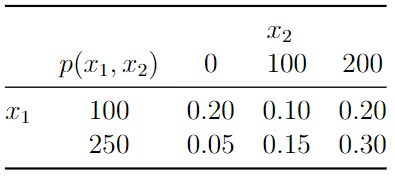
\includegraphics[width=0.2\textwidth,height=\textheight]{joint_pmf.PNG}

Then, for example, the probability the customer's auto deductible is 250 and home deductible is 100 is \(P(X_1 = 250, \, X_2 = 100) = p(250,100) = 0.15\).

In other cases joint PMFs may be derived using counting rules as the following example illustrates.

Example: Previously we used counting rules to find the PMF of the number of heads (or tails) in \(n\) flips of a coin with heads probability of \(p\) (usually \(p=1/2\)). That PMF is \(p(x) = {n \choose x}p^x (1-p)^{n-x}\). Now, suppose we roll a fair, six-sided die \(n\) times, and let \(X_1\) denote the number of 1's and \(X_2\) denote the number of 2's. What is the PMF of the probability we get \(x_1\) 1's and \(x_2\) 2's?

Solution: The chance of rolling a 1 is 1/6, and so is the chance of rolling a 2. So, provided \(x_1 + x_2 \leq n\) we have \((\tfrac16)^{x_1}(\tfrac16)^{x_2}(\tfrac46)^{n-x_1-x_2}\) probability of any string of rolls of \(x_1\) 1's, \(x_2\) 2's, and remaining rolls. Then, we have to count the number of ways of arranging said strings of rolls, and for this we use the formula for counting arrangements of distinguishable and indistinguishable objects --- that is, \(\frac{n!}{x_1! x_2! (n-x_1 -x_2)!}\). Therefore, the PMF is given by
\[p(x_1, x_2) = \frac{n!}{x_1! x_2! (n-x_1 -x_2)!}(\tfrac16)^{x_1}(\tfrac16)^{x_2}(\tfrac46)^{n-x_1-x_2}\]

\hypertarget{marginal-pmfs}{%
\subsection{Marginal PMFs}\label{marginal-pmfs}}

Given a joint PMF \(p(x_1, x_2)\) for r.v.'s \((X_1, X_2)\) we can \emph{marginalize} to either r.v., meaning we can compute the probabilities associated with just one of them. The ways we do this is by the law of total probability that we previously used to find probabilities of events using partitions. The marginal PMF of \(X_1\) given \(p(x_1, x_2)\) is given by
\[p(x_1) = \sum_{x_2} p(x_1, \, x_2) = \sum_{x_2} P(X_1 = x_1, \, X_2 = x_2).\]
What we're doing here is partitioning the event \(\{X_1 = x_1\}\) by values of \(X_2\), i.e.,
\[\{X_1 = x_1\} = \bigcup_{x_2}\{\{X_1 = x_1\}\cap\{X_2 = x_2\}\}.\]
Example: The marginal PMF of auto deductible is given by
\[p(100) = p(100,0)+p(100,100)+p(100,200) = 0.20+0.10+0.20=0.50\]
\[p(250) = p(250,0)+p(250,100)+p(250,200) = 0.05+0.15+0.30=0.50\]

Example: In the die rolling example above we could find the PMF of the number of 1's by using the general formula. On the other hand it's easier if we recognize that the experiment in which we roll a die \(n\) times and record the number of 1's is equivalent to a coin-slipping experiment with a biased/unfair coin. Then, it must be that the PMF is
\[p(x_1) = {n \choose x_1}(\tfrac16)^{x_1}(\tfrac56)^{n-x_1}.\]

\hypertarget{conditional-pmfs}{%
\subsection{Conditional PMFs}\label{conditional-pmfs}}

The conditional PMF \(p(x_1|x_2)\) assigns probabilities to the events \(\{X_1 = x_1\}\) within the sample space \(\mathcal{S}\cap \{X_2 = x_2\}\). Since probabilities of discrete random variables behave just like probabilities of events, we have
\[p(x_1|x_2) = \frac{p(x_1, \, x_2)}{p(x_2)},\]
i.e., the conditional PMF of \(X_1\) given \(X_2 = x_2\) is the ratio of the joint PMF to the marginal PMF of \(X_2\).

Example: The conditional PMF of home deductible given auto deductible is given by the following table. And, notice the conditional PMF sums to 1 across rows because the rows represent the conditional sample spaces.

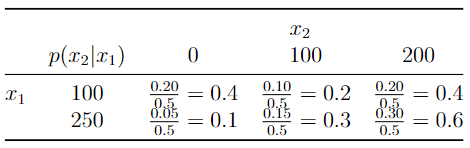
\includegraphics[width=0.4\textwidth,height=\textheight]{cond_pmf.PNG}

Example: Using the formula, we can compute the conditional PMF of the number of 2's in \(n\) dice rolls given the number of 1's (\(X_2\) given \(X_1\)).\\
\begin{align*}
p(x_2|x_1) &= \frac{\frac{n!}{x_1! x_2! (n-x_1 -x_2)!}(\tfrac16)^{x_1}(\tfrac16)^{x_2}(\tfrac46)^{n-x_1-x_2}}{{n \choose x_1}(\tfrac16)^{x_1}(\tfrac56)^{n-x_1}}\\
& = \frac{\frac{n!}{x_1! x_2! (n-x_1 -x_2)!}(\tfrac16)^{x_1}(\tfrac16)^{x_2}(\tfrac46)^{n-x_1-x_2}}{\frac{n!}{x_1!(n-x_1)!}(\tfrac16)^{x_1}(\tfrac56)^{n-x_1}}\\
& = \frac{(n-x_1)!}{x_2!(n-x_1-x_2)!}(\tfrac16)^{x_2}(\tfrac46)^{n-x_1-x_2}(\tfrac65)^{n-x_1}\\
&=\frac{(n-x_1)!}{x_2!(n-x_1-x_2)!}(\tfrac14)^{x_2}(\tfrac45)^{n-x_1}\\
& = \frac{(n-x_1)!}{x_2!(n-x_1-x_2)!}(\tfrac14)^{x_2}(\tfrac45)^{n-x_1-x_2}(\tfrac{4}{5})^{x_2}\\
& = \frac{(n-x_1)!}{x_2!(n-x_1-x_2)!}(\tfrac15)^{x_2}(\tfrac45)^{n-x_1-x_2}
\end{align*}
In other words, the conditional distribution is the same as the probability of \(x_2\) 2's in \(n-x_1\) rolls of a fair five-sided die with no 1-side!

\hypertarget{independence-of-discrete-random-variables}{%
\subsection{Independence of discrete random variables}\label{independence-of-discrete-random-variables}}

Two random variables \(X_1\) and \(X_2\) are independent if their conditional PMF (either one) is equal to the corresponding marginal PMF. This implies the product rule holds, and that their Joint PMF is the product of their marginal PMFs. That is,

\[p(x_1|x_2) = p(x_1)\quad\text{or, equivalently}\quad p(x_1,x_2)=p(x_1)p(x_2), \quad \forall (x_1,x_2).\]

Example: Let \(X_1\) and \(X_2\) denote score ranges for two players on a bowling team. suppose that if the player scores less than 100 they denote it with a zero, between 100 and 200 a 1 and better than 200 a 3. Determine whether their performances are independent given their joint PMF:

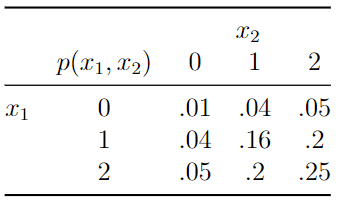
\includegraphics[width=0.2\textwidth,height=\textheight]{joint_pmf_ind.PNG}

By summing over the rows we obtain the marginal PMF of \(X_1\), given by \(p(x_1) = 0.1,\, 0.4,\, 0.5\) for values \(0\), 1, and 2, respectively. Summing over columns we find the same marginal PMF for \(X_2\). Then, we have \(p(0,0) = 0.01 = 0.1\times 0.1 = p_{x_1}(0)p_{x_2}(0)\), \(p(1,0) = 0.04 = 0.4\times 0.1 = p_{x_1}(1)p_{x_2}(0)\), etc. If we check each of the 9 joint PMF values, we find that in \textbf{every case} the joint PMF equals the product of marginal PMF values. Conclude \(X_1\) and \(X_2\) are independent.

\hypertarget{expectations-involving-multiple-discrete-random-variables}{%
\subsection{Expectations involving multiple discrete random variables}\label{expectations-involving-multiple-discrete-random-variables}}

Let \(g\) be a function involving two random variables \(g:(X_1,X_2)\mapsto \mathbb{R}\). Then, the expectation of \(g(X_1,X_2)\) is given by
\[E(g(X_1,X_2)) = \sum_{x_1,x_2} g(x_1,x_2)p(x_1,x_2).\]

The covariance of \(X_1\) amd \(X_2\), denoted \(Cov(X_1,X_2)\) is defined \(E[(X_1 - E(X_1))(X_2 - E(X_2))]\) where \(E(X_1)\) and \(E(X_2)\) are the marginal expectations, i.e., \(E(X_1) = \sum_{x_1} x_1 p(x_1)\). Covariance may be equivalently defined \(Cov(X_1, X_2) = E(X_1X_2)-E(X_1)E(X_2)\). If \((X_1,X_2)\) are independent, then \(Cov(X_1,X_2) = 0\).

Example: Find the covariance of auto and home deductibles.
The marginal distribution of home deductible is \(p(0) = 0.25\), \(p(100) = 0.25\), and \(p(200) = 0.50\). Then, the mean values of \(X_1\) and \(X_2\) are \(E(X_1) = 100*0.5 + 250 * 0.5 = 175\) and \(E(X_2) = 125\). The expectation of their product is
\[E(X_1X_2) = 0*100*0.2 + 100*100*0.1 + 100*200*0.2 + 0.*250*0.05 + 100*250*0.15 + 200*250*0.30=23750\]
Their covariance is \(23750-175*125 = 1875\).

Like the variance, the covariance has units equal to the product of the units of \(X_1\) and \(X_2\), which may or may not be interpretable. A unitless alternative to covarianceis \emph{correlation} which divides covariance by the product of standard deviations of the random variables:
\[Corr(X_1, X_2) = \frac{Cov(X_1,X_2)}{\sigma_{X_1}\sigma_{X_2}}.\]
Like covariance, correlation is zero for independent random variables. Unlike covariance, correlation is always between -1 and 1 and has no units. This gives it a meaningful scale for interpretation across applications.

Example: Find the correlation of auto and home deductibles.
We need the variances of the auto and home deductibles, which we can compute by finding the second raw moments.
\[E(X_1^2) = 100^2*0.5 + 250^2 * 0.5 = 36250\]
So, \(\sigma_{X_1}^2 = 36250-175^2 = 5625\). And,
\[E(X_2^2) = 100^2*0.25 + 200^2 * 0.5 = 22500\]
so that \(\sigma_{X_2}^2 = 22500 - 125^2 = 6875\).
Their correlation is \(1875/(\sqrt{5625*6875}) \approx 0.3015\).

\hypertarget{jointly-distributed-continuous-random-variables}{%
\section{Jointly distributed continuous random variables}\label{jointly-distributed-continuous-random-variables}}

Analogously to univariate continuous r.v.'s, the joint distribution of two (or more) continuous r.v.'s is characterized by its joint PDF \(f(x_1, x_2)\), and corresponding joint CDF \(F(x_1, x_2)\) which determine joint probabilities via integration:
\[P(X_1\leq x_1, X_2\leq x_2) =: F(x_1,x_2) = \int_{-\infty}^{x_1}\int_{-\infty}^{x_2}f(x_1,x_2)\,dx_2\,dx_1.\]
Example: A business takes both online and in-person orders. Let \(X_1\) and \(X_2\) be the waiting times for the next two orders to be placed. Suppose
\[f(x_1,x_2) = 2e^{-x_1-x_2}, \,\,0<x_1<x_2<\infty.\]
Find \(P(X_1\leq 1, X_2\leq 2)\).\\
\begin{align*}
P(X_1\leq 1, X_2\leq 2) &= F(1,2) = \int_0^1\int_{x_1}^2 2e^{-x_1-x_2} \,dx_2\, dx_1\\
& = 2\int_0^1 e^{-x_1}\left[\int_{x_1}^2 e^{-x_2} \,dx_2\right]\, dx_1\\
& = 2\int_0^1 e^{-x_1} \left[ - e^{-x_2}|_{x_1}^2\right]dx_1\\
& = 2\int_0^1 e^{-x_1}(e^{-x_1} - e^{-2})dx_1\\
& = 2\int_0^1 e^{-2x_1} - e^{-x_1-2}dx_1\\
& = 2[-\tfrac12 e^{-2x_1} + e^{-x_1-2}]|_{0}^1\\
& = -e^{-2}+2e^{-3}+e^{-0}-2e^{-2}\\
& \approx 0.693568
\end{align*}

\hypertarget{marginal-densities}{%
\subsection{Marginal densities}\label{marginal-densities}}

Given a joint PDF of \((X_1, X_2)\) the marginal PDFs determine the probabilities associated with each r.v. individually. That is, for \(X_1\)
\[f_{X_1}(x_1) = \int_{-\infty}^\infty f(x_1, x_2) dx_2\]
is the marginal density of \(X_1\) so that integration of the marginal PDF provides
\[P(X_1\leq x_1) = F_{X_1}(x_1) = \int_{-\infty}^{x_1} f_{X_1}(t)dt.\]
Example: For the above joint probability density of waiting times we get the marginal density of \(X_1\):
\begin{align*}
f_{X_1}(x_1) &=  2e^{-x_1}\int_{x_1}^{\infty}e^{-x_2}dx_2\\
& = 2e^{-x_1}[-e^{-x_2}]|_{x_1}^\infty\\
& = 2e^{-x_1}[0 + e^{-x_1}]\\
& = 2e^{-2x_1}, \quad x_1>0.
\end{align*}

From the marginal PDF we can compute any kind of marginal expectation we want, like \(E(X_1)\), \(V(X_1)\), or \(M_{X_1}(t)\).

Example: The moment generating function of the first arrival time is given by
\begin{align*}
M_{X_1}(t) &= \int_{0}^\infty 2e^{tx}e^{-2x}dx\\
& = \int_{0}^\infty 2e^{-x(2-t)}dx \\
& = 2\frac{e^{-x(2-t)}}{-(2-t)}|_{0}^\infty\\
& = \frac{2}{2-t}, \quad t<2.
\end{align*}
And, the first (raw) moment then equals
\begin{align*}
E(X_1) &= \frac{d}{dt}[\frac{2}{2-t}]|_{t=0}\\
&= \frac{2}{(2-t)^2}|_{t=0}\\
& = 1/2.
\end{align*}

\hypertarget{conditional-densities}{%
\subsection{Conditional densities}\label{conditional-densities}}

Given the joint and marginal densities \(f(x_1, x_2)\) and \(f_{X_1}(x_1)\) we can define the conditional density of \(X_2\) given \(X_1=x_1\) by
\[f(x_2|x_1) = \frac{f(x_1, x_2)}{f_{X_1}(x_1)}\]
which defines the probabilities
\[P(X_2\leq x_2|X_1=x_1) = \int_{-\infty}^{x_2} f(t|x_1)dt.\]

Example: Given the first order arrives at time 1, what is the probability the second order arrives before time 2?
\[f(x_2|x_1) = \frac{2e^{-x_1-x_2}}{2e^{-2x_1}} = \frac{e^{-x_2}}{e^{-x_1}}, \quad x_2>x_1.\]

\begin{align*}
P(X_2\leq 2|X_1=1) &= \int_{1}^2 \frac{e^{-x_2}}{e^{-1}}dx_2\\
&= e^{1}[-e^{-x_2}]|_1^2\\
& = e^{1}(e^{-1}-e^{-2})\\
& = 1-e^{-1}\\
& \approx 0.63212
\end{align*}

Example: Find the mean of the second arrival time, given the first arrival time is 1.

\begin{align*}
E(X_2|X_1=1) &= \int_{1}^\infty x_2\frac{e^{-x_2}}{e^{-1}}dx_2\\
& = e^{1}\int_{1}^\infty x_2e^{-x_2}dx_2\\
& = e^1[-x_2e^{-x_2}|_1^\infty + \int_1^\infty e^{-x_2}dx_2] \quad \text{use by-parts}\\
& = e^1[e^{-1} - e^{-x_2|_1^\infty}]\\
& = 2
\end{align*}

\hypertarget{independence-of-jointly-distributed-continuous-r.v.s}{%
\subsection{Independence of jointly-distributed continuous r.v.'s}\label{independence-of-jointly-distributed-continuous-r.v.s}}

Random variables \(X_1\) and \(X_2\) are independent if \(f(x_1|x_2) = f_{X_1}(x_1)\) for every \(x_2\); or, equivalently, if \(f(x_2|x_1) = f_{X_2}(x_2)\) for every \(x_1\).

Example: A randomly selected student's verbal score \(X_1\) and quantitative score \(X_2\) on a college entrance exam have the joint PDF
\[f(x_1, x_2) = \tfrac25 (2x_1+3x_2), \quad 0\leq x_1\leq 1, \, 0\leq x_2\leq 1.\]
Are they independent?

Solution:
The marginal density of \(X_1\) is given by
\[\int_{0}^1 \tfrac25 (2x_1+3x_2)dx_2 = \tfrac25[2x_1x_2+1.5x_2^2]|_0^1 = \tfrac45 x_1 + 1.5\]

The marginal density of \(X_2\) is given by
\[\int_{0}^1 \tfrac25 (2x_1+3x_2)dx_1 = \tfrac25[\tfrac12x_1^2+3x_2x_1]|_0^1 = \tfrac15  + \tfrac65 x_2.\]
The conditional density of \(X_2|X_1=x_1\) is
\[\frac{\tfrac25(2x_1+3x_2)}{\tfrac45 x_1+1.5} \ne f_{X_2}(x_2).\]
They are not independent.

Example: For the waiting time distribution above, the marginal density of \(X_2\) equals
\begin{align*}
f_{X_2}(x_2) &= \int_0^{x_2} 2e^{-x_1-x_2}dx_1\\
& = 2e^{-x_2} - 2e^{-2x_2}, \quad x_2>0.
\end{align*}

We previously found the conditional density \(f(x_2|x_1) = \frac{e^{-x_2}}{e^{-x_1}}, \,\,x_2>x_1\). These two densities---the conditional and the \(X_2-\)marginal--- are not equal, so \(X_1\) and \(X_2\) are not independent. Of course, it is clear they are dependent just by looking at their domain---since \(x_2\geq x_1\) they must be dependent.

\hypertarget{expectations-involving-more-than-one-continuous-r.v.}{%
\subsection{Expectations involving more than one continuous r.v.}\label{expectations-involving-more-than-one-continuous-r.v.}}

As in the discrete case, we can compute expectations of functions of two or more continuous r.v.'s:
\[E(g(X_1,X_2)) = \int_{-\infty}^\infty\int_{-\infty}^\infty g(x,y)f(x,y) dxdy.\]

Example: Using the order times example we compute \(Cov(X_1, X_2)\), the covariance of the order times of the first and second orders:
\begin{align*}
E(X_1X_2) &= \int_0^\infty \int_{x_1}^\infty 2x_1x_2e^{-x_1-x_2} dx_2 dx_1\\
& = 2\int_0^\infty x_1e^{-x_1} \left [\int_{x_1}^\infty x_2e^{-x_2}dx_2\right ] dx_1 \quad \text{use by-parts}\\
& \text{set }u=x_2\, du = dx_2\, dv = e^{-x_2}\, v = -e^{-x_2}\, \\
& = 2\int_0^\infty x_1e^{-x_1} \left [uv|_{x_1}^\infty - \int_{x_1}^\infty vdu \right] dx_1\\
& = 2\int_0^\infty x_1e^{-x_1}(1+x_1)e^{-x_1}dx_1 \, \text{ have to do by-parts twice...}\\
& = 1
\end{align*}

The mean of \(X_1\) is
\begin{align*}
E(X_1) &= \int_0^{\infty} x_12e^{-2x_1} dx_1\\
& = 1/2.
\end{align*}

Then,
\begin{align*}
E(X_2) &= \int_0^\infty 2x_2(e^{-x_2}-e^{-2x_2}) dx_2 \\
& = 3/2 \quad \text{apply integratioon by parts}
\end{align*}

The covariance of \(X_1\) and \(X_2\) is \(1 - (3/2)(1/2) =1/4\).

\hypertarget{special-discrete-distributions}{%
\chapter{Special Discrete Distributions}\label{special-discrete-distributions}}

\hypertarget{bernoulli-distribution}{%
\section{Bernoulli Distribution}\label{bernoulli-distribution}}

\(X\) is a Bernoulli random variable if it only takes values \(0\) or \(1\). Denoting \(p:=P(X=1)\) the PMF can be written \(p(x) = p^x(1-p)^{1-x}\). The mean and variance are easily found to be \(E(X) = p\) and \(V(X) = p(1-p)\). The MGF is \(M_X(t) = 1-p+pe^t\).

The Bernoulli distribution can describe two different experiments:
1. One random sample is taken from a finite population of size \(N\) of \(Np\) 1's and \(N(1-p)\) 0's (or any binary attribute), it's value is recorded, and it is then replaced.
2. One random sample is taken, without replacement, from an infinite population of 1's and 0's in proportions of \(p\) and \(1-p\).

\hypertarget{categorical-distribution}{%
\section{Categorical Distribution}\label{categorical-distribution}}

The categorical distribution generalizes the Bernoulli distribution to more than two values (more than two categories). \(X\) is a categorical random variable if it takes values in a finite set of integers, usually \(\{1,2,\ldots,k\}\) for \(k\geq 3\). Let \(p_i:=P(X=i)\) so that \(0\leq p_i\leq 1\) and \(\sum_{i=1}^k p_i = 1\). Note we only need specify \(p_1,\ldots p_{k-1}\) and then \(p_k = 1- \sum_{i=1}^{k-1}p_i\). The categorical PMF is
\[p(x_1,x_2,\ldots,x_{k-1}) = \prod_{i=1}^{k} p_i^{x_i} = \left\{(1-\sum_{i=1}^{k-1} p_i)^{1-\sum_{i=1}^{k-1} x_i}\right\} \prod_{i=1}^{k-1} p_i^{x_i}.\]

The categorical distribution can describe the same two types of experiments as the Bernoulli, except where the number of categories/values is now \(k\) rather than \(2\).

\hypertarget{binomial-distribution}{%
\section{Binomial distribution}\label{binomial-distribution}}

If \(X_1,X_2,\ldots, X_n\) is a random sample of \(n\) Bernoulli random variables with parameter \(p\), then \(Y = \sum_{i=1}^n X_i\) is a Binomial random variable with PMF
\[p(y) = {n \choose y}p^y(1-p)^{n-y}, \,\, y\in \{0, 1,\ldots, n\}.\]

The easiest way to determine moments of the Binomial distribution is to consider its MGF. Using the fact the Binomial is a sum of independent and identically distributed (same \(p\)) Bernoulli r.v.'s we have
\begin{align*}
E(e^{tY}) & = E(e^{t\sum X_i}) \\
& = E\left\{\prod_{i=1}^n e^{t X_i}\right\}\\
& \stackrel{ind.}{=} \prod_{i=1}^n (1-p + pe^t)\\
& = (1-p + pe^t)^n.
\end{align*}
Then, by differentiating once and twice:
\[E(Y) = npe^t(1-p + pe^t)^{n-1}|_{t=0} = np\]
\[E(Y^2) = npe^t(1-p + pe^t)^{n-1} + npe^t(n-1)pe^t((1-p + pe^t)^{n-2})|_{t=0} = np+(np)^2-np^2\]
\[V(Y) = np(1-p).\]

The Binomial distribution describes the outcomes of a repeated random sampling of Bernoulli r.v.'s. For example, in a poll of eligible voters with a binary ``yes'' or ``no'' vote a Bernoulli random variable represents one voter's outcome/vote and a Binomial random variable represents the sum of outcomes in the entire poll of \(n\) voters. Often, rather than the sum total we are interested in the sample proportion of yes/no votes, which is the transformation \(Z = Y/n\). Probabilities of \(Z\) are easily deduced from \(Y\) by \(P(Z = z) = P(Y = nz)\). Likewise, \(E(Z^q) = \frac{1}{n^q}E(Y)\) for positive integers \(q\). For example, the mean and variance of the sample proportion is \(E(Z) = p\) and \(V(Z) = \frac{p(1-p)}{n}\).

\hypertarget{multinomial-distribution}{%
\section{Multinomial Distribution}\label{multinomial-distribution}}

Let \(X_i\) be a categorical random variable encoded as a binary vector in \(\mathbb{R}^k\) with \(\|X_i\|_1 = 1\). That is, \(X_i\) is a vector of zeroes and one 1 at the \(j^{th}\) index if \(X_i\) takes value \(j \in \{1,\ldots, k\}\). This is a different representation than simply taking \(X_i\) equal to its category, as represented by an integer. Then, if \(X_1, X_2, \ldots, X_n\) is a random sample (a set of independent and identically distributed) categorical random variables (as represented by binary \(k-\)vectors), then \(Y = \sum_{i=1}^n X_i\) is a Multinomial random variable. Note \(Y\) is a \(k0-\)vector with integer entries representing the counts of each category appearing in the random sample. So, the Multinomial is analogous to the Binomial as the categorical is to the Bernoulli. The PMF of \(Y\) is

\[p(y_1, y_2, \ldots, y_{k}) = \frac{n!}{y_1!\times y_2!\times \cdots \times y_k!}p_1^{y_1}\times \cdots \times p_k^{y_k}\]
where \(n = \sum_{i=1}^k y_i\), \(p_k = 1 - \sum_{i=1}^k p_i\).

Using the representation of the Multinomial in terms of sums of categorical random variables helps in computing moments. Let's compute the covariance of \(Y_\ell\) and \(Y_j\), which represent the counts of categories \(\ell\) and \(j\). For each count, write \(Y_j = \sum_{i=1}^nX_{ij}\), the sum of the \(j^{th}\) index of the X categorical random variable vectors. Then,
\begin{align*}
E(Y_\ell Y_j) &= E\{(\sum_{i=1}^n X_{i\ell})(\sum_{i=1}^n X_{ij})\}\\
& = E(\sum_{i=1}^n X_{i\ell}X_{ij}) + E(\sum_{i=1,i\ne i'}^n X_{i\ell}X_{i'j})\\
& = E(0) + E(\sum_{i=1,i\ne i'}^n X_{i\ell}X_{i'j})\\
& \stackrel{ind.}{=}  \sum_{i=1,i\ne i'}^n E(X_{i\ell})E(X_{i'j})\\
& = n(n-1)p_\ell p_j.
\end{align*}
The marginal expectations are easier to compute:
\[E(Y_\ell) = E\left\{\sum_{i=1}^n X_{i\ell}\right\} = np_\ell.\]
Therefore, the covariance is
\[Cov(Y_\ell, Y_j) = -np_\ell p_j,\]
which makes sense --- for \(n\) samples if there are more samples in category \(\ell\) then there necessarily are fewer in category \(j\), and vice versa.

The Multinomial distribution is special for the fact its marginal and conditional distributions are also multi/binomial. Consider the marginal distribution of the first category count \(Y_1\). Using the total probability formula, we can compute its marginal probabilities:
\[P(Y_1 = y_1) = \sum_{\mathbb{Y}}P(Y_1 = y_1, Y_2 = y_2, Y_3 = y_3, \ldots,Y_k = y_k),\]
where \(\mathbb{Y} = \{(y_2, \ldots, y_k): n-y_1 =\sum_{2}^k y_j\}\). In other words,
\[P(Y_1 = y_1) = P(Y_1 = y_1, \sum_2^k Y_j = n - y_1).\]
This reveals that the marginal probability of \(Y_1\) is a Binomial probability---the only ``categories'' that matter to the computation are ``1'' and ``not 1''. Therefore, \(Y_j \sim\)Binomial\((n,p_j)\) for \(j \in \{1,\ldots,k\}\).

Given the one-dimensional marginal distributions are Binomial, we can compute the conditional PMF of \(Y_2,\ldots, Y_k|Y_1 = y_1\) as the ratio of joint to marginal PMFs:

\begin{align*}
p(y_2, \ldots, y_k|y_1) &= \frac{\frac{n!}{y_1!\times \cdots \times y_k!} p_1^{y_1}\times \cdots \times p_k^{y_k}}{ \frac{n!}{y_1! (n-y_1)!} p_1^{y_1}(1-p_1)^{n-y_1}}\\
& = \frac{(n-y_1)!}{y_2!\times \cdots y_k!}\left(\frac{p_2}{1-p_1}\right)^{y_2}\times \cdots \times \left(\frac{p_k}{1-p_1}\right)^{y_k}.
\end{align*}

\hypertarget{hypergeometric-distribution}{%
\section{Hypergeometric distribution}\label{hypergeometric-distribution}}

The Hypergeometric distribution describes sampling from a finite population without replacement. Traditionally, the distribution describes binary outcomes, but the idea is generalizeable.

Suppose there are \(n = n_1 + n_2\) individuals, \(n_1\) 1s and \(n_2\) 0s. If \(k\) individuals are randomly selected without replacement, then the probability \(j\) of them are 1s is
\[P(X = j) = p(j) = \frac{{n_1 \choose j}{n_2 \choose k-j}}{{n \choose k}}, \, \, 0\leq j\leq \min(k,n_1).\]

The calculations of moments of the Hypergeometric distribution requires repeated use of the Binomial Theorem, and does not provide much insight about the distribution, but the formulas for the Hypergeometric mean and variance are insightful, so we include them here.
\[E(X) = k\frac{n_1}{n}\quad V(X) = k\frac{n_1}{n}\frac{n_2}{n}\frac{n-n_1}{n-1}.\]
The mean of \(X\) is very similar to the mean of a Binomial r.v. In this case the population proportion of 1s is exactly \(n_1/n\), which is analogous to \(p\) in the Binomial case, so the formula is virtually the same. On the other hand, the variance for the Hypergeometric is like \(np(1-p)\) times a ``correction term'' \(\frac{n-n_1}{n-1}\). We can understand the correction term as accounting for the finite-ness of the population/sampling without replacement versus sampling with replacement, as in the case of a Binomial experiment. If \(n\) is large relative to \(n_1\), then this term is negligible, and there is little difference between the variances of the two distributions.

Consider extending the hypergeometric to more than two categories. Let \(Y_1\), \(Y_2\), and \(Y_3\) denote the counts of observations in each of three possible categories. These are sums of categorical random variable vectors sampled without replacement. Then,

\[P(Y_1 = y_1, Y_2 = y_2, Y_3 = y_3) = \frac{{n_1\choose y_1}{n_2\choose y_2}{n_3\choose y_3}}{{n \choose y}}\]
where \(n = n_1+n_2+n_3\) represent the population category counts, \(y_1 + y_2 + y_3 = y \leq n\), and \(0\leq y_i\leq n_i\) for \(i=1,2,3\).

\hypertarget{negative-binomial-distribution}{%
\section{Negative Binomial Distribution}\label{negative-binomial-distribution}}

Let \(X_1, X_2, \ldots\) represent independent, identically distributed Bernoulli r.v.'s and define \(Y\) to be the number of 1's observed when the \(k^{th}\) 0 is observed; \(k\) is a fixed parameter. Then, the PMF of \(Y\) is
\[p(y) = {k + y - 1 \choose k-1}(1-p)^kp^{y}, \, y\geq 0.\]
We say \(Y\) is a Negative Binomial r.v. In the special case that \(k=1\) \(Y\) is called a Geometric r.v. and the PMF simplifies to
\[p(y) = (1-p)p^y\]
The Negative Binomial is closely related to the binomial distribution. Both involve sequences of iid Bernoulli r.v.'s, but count different types of outcomes. The Binomial counts ``successes'' while the Negative Binomial counts ``trials'' until the \(k^{th}\) failure. Notice that there is a built-in conditioning inherent in the negative binomial because we know the last trial is a failure. This accounts for the ``counting term'' appearing in the PMF---the last trial is fixed as a failure, so there are only the previous \(k+y - 1\) trials that can be arranged in any order.

The Negative Binomial for \(k\) ``failures'' can be represented as a sum of \(k\) independent Geometric r.v.'s, much like the Binomial is a sum of \(n\) Bernoulli r.v.'s. This makes computing moments much simpler. If \(X\) is a Geometric r.v., then
\[E(X) = \sum_{x=0}^\infty x \, p^x (1-p) = \frac{(1-p)p}{(1-p)^2} = \frac{p}{1-p}.\]
Then, if \(Y\) is Negative Binomial with parameter \(k\), \(E(Y) = \frac{kp}{1-p}\).

\hypertarget{poisson-distribution}{%
\section{Poisson Distribution}\label{poisson-distribution}}

Consider an experiment in which you count the number of ``events'' that happen since time zero to time \(t>0\). For example, you might count shooting stars from your campsite at Big Creek State Park. This doesn't sound like other experiments we've discussed. For one, how would you compute \(P(X_t = 5)\), the chance the number of shooting stars observed by time \(t\) is 5? It's not clear how a counting argument would apply to this situation. As we'll show below, with a few assumptions we can use a counting argument to derive this probability, and, once again, the Bernoulli distribution is key\ldots{}

For a little more structure, let's assume the following:
1. If we consider a very small time interval, \((0, \delta t)\) for a fixed \(t>0\) and a small number \(\delta>0\) we assume no more than one event can be observed in the interval. Essentially, this means events cannot occur \emph{simultaneously}.
2. The probability of one event in and interval of time length \(\delta t\) is proportional to \(\delta t\), that is, the probability equals \(\lambda \delta t\) for some constant \(\lambda >0\).
3. For any two disjoint time intervals, the counts of events in those two intervals are independent.

These assumptions allow us to make the following argument: the time interval \((0,t)\) can be partitioned into the union of disjoint intervals
\[(0,t) = \bigcup_{j=1}^{1/\delta} ((j-1)\delta t, \, j\delta t).\]
And, the probability of \(k\) events in \((0,t)\) is now a Binomial r.v.
\[\text{``}P(X = k) = {1/\delta\choose k} (\lambda \delta t)^k (1- \lambda \delta t)^{1/\delta - k}.\text{"}\]
I've written the previous probability in quotes for a couple of reasons\ldots{} First, since \(1/\delta\) may not be an integer, it doesn't really make sense. Second, \(\delta\) is not really a constant. Our assumption truly is that no two events happen simultaneously, which implies our treatment of intervals as Bernoulli random variables is only valid in a limiting sense as the width of the intervals is taken to be arbitrarily small. We can incorporate this limit by evaluating the limit of the PMF in quotes above as \(\delta \rightarrow 0\). Equivalently, we can evaluate the limit of the corresponding Binomial MGF as \((1/\delta)\rightarrow \infty\), which is slightly easier. Recall the Binomial MGF in this context is
\[M_X(u) = (1- \lambda \delta t + \lambda \delta t e^u)^{1/\delta}.\]
Then, its limit satisfies (defining \(v = 1/\delta\))
\begin{align*}
\lim_{v \rightarrow \infty} \left(1+ \frac{\lambda t(e^u -1)}{v}\right)^{v}\\
& = e^{\lambda t(e^u - 1)}
\end{align*}
using the fact \(\lim_n\rightarrow \infty (1+x/n)^n = e^x.\)
This function is the MGF of the Poisson distribution, and has corresponding PMF
\[p(x) = \frac{(\lambda t)^x e^{-\lambda t}}{x!},\, x=0,1,\ldots\]

\hypertarget{example-1-poisson-process}{%
\subsection{Example 1: Poisson process}\label{example-1-poisson-process}}

Shoppers enter Hyvee according to a Poisson process with intensity \(\lambda = 6\) per minute. What is the chance that in the next 15 seconds either 0, 1, or 2 customers enter?

Solution: First, find the intensity for a 15 second period, \(6\) per minute means \(1.5\) per 15 seconds. Then, compute

\[p(0)+p(1)+p(2) = \frac{\lambda^0e^{-\lambda}}{0!}+\frac{\lambda^1e^{-\lambda}}{1!}+\frac{\lambda^2e^{-\lambda}}{2!}\]
\[e^{-1.5}\left\{1+a.5 + \frac{1.5^2}{2}\right\}\]
\[ \approx 0.809\]

\hypertarget{example-2-poisson-approximation-to-binomial}{%
\subsection{Example 2: Poisson approximation to Binomial}\label{example-2-poisson-approximation-to-binomial}}

Let \(X\sim Binomial(n,p)\). When the number of trials is ``large'' and the Bernoulli success probability \(p\) is small, \(p(x)\) can be approximated by the Poisson PMF \(p(y)\) where \(Y\sim Poisson(\lambda = np)\). A rule of thumb provided by the Freund textbook says the approximation is good when \(n\geq 20\) and \(p\leq 0.05\).

Suppose in a population of drivers about \(5\%\) will have an accident in the coming year. Let \(X\) be the number of accidents among a random sample of 150 of these drivers. Find \(p(5)\), the probability there will be 5 accidents among the sampled drivers. Use the Binomial and its Poisson approximation and compare the answers.

Solution:
\[p_X(5) = {150 \choose 5}(0.05)^5(0.95)^{145} = dbinom(5,150,0.05) \approx 0.109. \]
Let \(Y \sim Poisson(7.5)\).
\[p_Y(5) = \frac{7.5^5 e^{-7.5}}{5!} = dpois(5,7.5) \approx 0.109. \]

\hypertarget{optional-derivation-of-the-poisson-pmf-using-differential-equations}{%
\section{Optional: Derivation of the Poisson PMF using differential equations}\label{optional-derivation-of-the-poisson-pmf-using-differential-equations}}

We begin with the same three assumptions as before: in a very small time intervals (of length \(\delta t\)) the number of events is Bernoulli with \(p=\lambda\delta t\), and counts in disjoint time intervals are independent.

Next, consider the probability of zero events in the time interval \((0, t+\delta t)\). This is equal the probability of no events in \((0,t)\) and no events in \((t, t+\delta t)\), two disjoint time intervals. We can write this probability as
\[P(0; t+\delta t) = P(0;t)(1-\lambda \delta t)\]
using the fact the probability in the second, small interval is Bernoulli. Rewrite this as
\[\frac{P(0;t+\delta t)-P(0;t)}{\delta t} = -\lambda P(0;t),\]
and, taking limits as \(\delta t \rightarrow 0\) we obtain the separable ODE
\[\frac{dP(0;t)}{dt} - \lambda P(0;t).\]
Integrating both sides we find
\[P(0;t) = Ce^{-\lambda t}\]
for a constant \(C>0\). The ``initial condition'' says \(P(0;0) = 1\) because no events can happen in a time interval of length zero, which implies \(C=1\).

So far we have found the probability of zero events in time interval \((0,t)\). What about generalizing this to \(n\) events? Use the same technique and represent the interval \((0, t+\delta t)\) as the union of \((0,t)\) and \((t, t+\delta t)\). For the probability there are \(n\) events in time \((0,t+\delta t)\) there are two possibilities: \(n-1\) events in \((0,1)\) and \(1\) in \((t, t+\delta t)\) or \(n\) events in \((0,t)\) and none in \((t, t+\delta t)\) and this happens with probability
\[P(n;t+\delta t)  = P(n;t)(1-\lambda \delta t) + P(n-1;t)\lambda\delta t.\]
Again, taking the limit as \(\delta t \rightarrow 0\) we obtain the ODE
\[\frac{d P(n;t)}{dt} + \lambda P(n;t) = \lambda P(n-1;t).\]
The ``integrating factor'' approach can be used to solve this ODE. The goal is to find a function \(g(t)\) such that
\[g(t)\left\{\frac{d P(n;t)}{dt} + \lambda P(n;t)\right\} = \frac{d}{dt}\{g(t)P(n;t)\}.\]
A little intuition suggests \(e^{\lambda t}\), which works. We have
\[\frac{d}{dt}\{e^{\lambda t}P(n;t)\} = \lambda e^{\lambda t}P(n-1;t).\]
Plugging in \(n=1\) we see that
\[\frac{d}{dt}\{e^{\lambda t}P(1;t)\} = \lambda e^{\lambda t}P(0;t) = \lambda e^{\lambda t}e^{-\lambda t} = \lambda.\]
And, integrating both sides above we get
\[e^{\lambda t}P(1;t) = \lambda t + C,\]
where \(C = 0\) is implied by the fact \(P(1;0) = 0\), the chance of 1 count in no time is zero.
So far, we have found \(P(0;t) = e^{-\lambda t}\) and \(P(1;t) = \lambda t e^{-\lambda t}\). For general \(n\), the idea is to repeat this argument inductively, assuming \(P(n;t) = \frac{(\lambda t)^n e^{-\lambda t}}{n!}\). For the inductive step, we need only show that assuming the above will show \(P(n+1;t) = \frac{(\lambda t)^{n+1} e^{-\lambda t}}{(n+1)!}\) and we're done. This follows from the differential equation:
\[\frac{d}{dt}\left\{e^{\lambda t}P(n+1;t)\right\} = \lambda e^{\lambda t}P(n;t) = \lambda e^{\lambda t} \frac{(\lambda t)^n e^{-\lambda t}}{n!} = \lambda \frac{(\lambda t)^n}{n!}.\]
Integrating both sides we obtain
\[e^{\lambda t}P(n+1;t) = \frac{(\lambda t)^{n+1}}{(n+1)!}+C\]
where, again, \(C=0\) follows from \(P(n+1;0) = 0\). Therefore, solving for \(P(n+1;t)\) we obtain
\[P(n+1;t) = \frac{(\lambda t)^{n+1}e^{-\lambda t}}{(n+1)!}\]
as claimed.

\hypertarget{special-continuous-distributions}{%
\chapter{Special Continuous Distributions}\label{special-continuous-distributions}}

\hypertarget{exponential-distribution}{%
\section{Exponential Distribution}\label{exponential-distribution}}

Let \(Y~\sim Poisson(\lambda t)\) be a Poisson process with intensity \(\lambda t\). Let \(X\) be the time until the next count/event is observed. Then, the probability \(X \geq t\) is the probability is takes at least \(t\) time for the next event, has probability
\[P(X > t) = P(\text{no events in }(0,t)) = P_Y(0;t) = \frac{(\lambda t)^0 e^{-\lambda t}}{0!} = e^{-\lambda t}.\]
The CDF of \(X\) then must be
\[F_X(x) = 1-P(X > x) = P(X\leq x) = 1-e^{-\lambda x},\]
and the PDF of \(X\) is
\[f_X(x) = \frac{d}{dx}F_X(x) = \lambda e^{-\lambda x}, \, x\geq 0.\]

We recognize this as the PDF of an \emph{Exponential random variable}. This derivation provides an important connection between the Exponential and Poisson (and, ultimately, Bernoulli) distributions: the waiting times of an Poisson process (with intensity \(\lambda t\)) are Exponentially distributed (with mean \(1/\lambda\)).

The MGF of the Exponential distribution is

\[M_X(t) = E(e^{tX})  = \int_{0}^\infty \lambda e^{-\lambda x(1-t/\lambda)}dx\]
\[ = \frac{\lambda e^{-\lambda x(1-t/\lambda)}}{-\lambda (1-t/\lambda)}|_0^\infty\]
\[ = \frac{1}{1-t/\lambda}, \text{ provided }t < \lambda.\]

Taking derivatives:
\[\frac{d}{dt}M_X(t) = \frac{1}{\lambda(1-t/\lambda)^2}, \]
and taking \(t = 0\) implies \(E(X) = 1/\lambda\).
And, again,
\[\frac{d^2}{dt^2}M_X(t) = \frac{2}{\lambda^2(1-t/\lambda)^3}\]
which implies \(E(X^2) = 2/\lambda^2\) and \(V(X) = 1/\lambda^2\).

\hypertarget{poisson-interarrival-times-are-iid-exponentiallambda}{%
\section{\texorpdfstring{Poisson Interarrival times are iid Exponential(\(\lambda\))}{Poisson Interarrival times are iid Exponential(\textbackslash lambda)}}\label{poisson-interarrival-times-are-iid-exponentiallambda}}

In this section we show that the subsequent times to events in a Poisson process are iid Exponential(\(\lambda\))-distributed. We prove this for only the first \(2\) such times, and hope the intuition is clear as to why the general case holds also.

Let \(X_1\) be the time to the first event. We have already shown this is \(Exp(\lambda)\). Let \(X_2\) be the additional (not total) time to the second event. Our strategy is to compute the joint probability funciton \(P(X_1 >x_1, X_2 >x_2)\) and note this is a product of the marginal probabilities \(P(X_1 >x_1)\) and \(P(X_2 >x_2)\), then we will have shown the claim. The easiest way to do this is to first consider the total times \(S_1 = X_1\) and \(S_2 = X_1 + X_2\).

Start by writing
\begin{align*}
F_{S_1, S_2}(s_1, s_2) &= P(S_1 \leq s_1, S_2 \leq s_2)\\
& = 1 - P(S_1 > s_1, S_2 > s_2) \\
&- P(S_1 \leq s_1, S_2 > s_2)\\
&P(S_1 > s_1, S_2 \leq s_2).
\end{align*}

Now, \(P(S_1 > s_1, S_2 > s_2)\) is the probability there are no events in \((0,s_1)\) and no more than 1 event in \((s_1, s_2)\). By the definition of the Poisson process, the counts in disjoint intervals are independent, so we have
\begin{align*}
P(S_1 > s_1, S_2 > s_2) & = P(Y((0, s_1)) = 0, \, Y((s_1, s_2))\leq 1)\\
& = P(Y((0, s_1)) = 0)P(Y((s_1, s_2))\leq 1)\\
& = \frac{(\lambda s_1)^0e^{-\lambda s_1}}{0!}\times\left\{ \frac{(\lambda (s_2-s_1))^0e^{-\lambda (s_2-s_1)}}{0!}+ \frac{(\lambda (s_2-s_1))^1e^{-\lambda (s_2-s_1)}}{1!}\right\}
\end{align*}

Similar arguments show:
\[P(S_1 \leq s_1, S_2 > s_2) = \lambda s_1 e^{-\lambda s_2}.\]
\[P(S_1 > s_1, S_2 \leq s_2) = e^{-\lambda s_1} - e^{-\lambda s_2}(1+\lambda(s_2 - s_1)).\]

Then,
\[F_{S_1, S_2}(s_1, s_2) = 1-e^{-\lambda s_1} - \lambda s_1 e^{-\lambda s_2}.\]
And, by differentiating once w.r.t. \(s_1\) and once w.r.t. \(s_2\) we obtain
\[f_{S_1, S_2}(s_1, s_2) = \lambda^2e^{-\lambda s_2}, \, 0<s_1<s_2.\]
Next,
\begin{align*}
P(X_1 > x_1, X_2 > x_2) &= P(S_1 > x_1, S_2-S_1 > x_2)\\
& = \int_{x_1}^\infty \int_{s_1 + x_2}^\infty \lambda^2 e^{-\lambda s_2}\,ds_2\,ds_1\\
& = e^{-\lambda x_1}e^{-\lambda x_2}.
\end{align*}
Notice this is a product of the marginal \(Exp(\lambda)\) probabilities \(P(X_1 > x_1) = e^{-\lambda x_1}\) and \(P(X_2 > x_2) = e^{-\lambda x_2}\).

\hypertarget{gamma-distribution}{%
\section{Gamma Distribution}\label{gamma-distribution}}

Let \(X_1, X_2, \ldots, X_n\) be a sequence of iid Exponential\((\lambda)\) r.v.'s. For example, these could be the successive waiting times of the next \(n\) events in a Poisson process with intensity \(\lambda t\). Then, the total waiting time for the next \(n\) events is \(Y = \sum_{i=1}^n X_i\). Using the MGF method, we see
\[M_Y(t) = E(e^{tY}) = E(e^{t \sum_{i=1}^n X_i}) \stackrel{ind.}{=}\prod_{i=1}^n M_{X_i}(t)\stackrel{iid}{=}M_X(t)^n = \left(\frac{1}{1-t/\lambda}\right)^n,\]
which is the MGF of a \emph{Gamma} random variable with two parameters: the shape (here \(n\)), and the rate (here \(\lambda\)). The Gamma distribution has PDF
\[f_Y(y) = \frac{\lambda^n}{\Gamma(n)}y^{n-1}e^{-\lambda y},\, y>0\]
where \(\Gamma(\cdot)\) denotes the ``Gamma'' function. If \(n\) is a positive integer \(\Gamma(n) = (n-1)!\). Note: the PDF can be derived from the MGF using the \textbf{inverse Laplace transform} but we'll not venture into these mathematical details here.

Using the fact the Gamma r.v. is a sum of iid Exponential r.v.'s we have
\[E(Y) = n/\lambda \quad\text{and}\quad V(Y) = n/\lambda^2.\]
In general, the shape parameter \(n\) need not be an integer, but if it is a fraction, then we lose the interpretation of the Gamma r.v. in terms of total waiting time.

\hypertarget{normal-gaussian-distribution}{%
\section{Normal (Gaussian) Distribution}\label{normal-gaussian-distribution}}

We have already seen how a limiting case of the Binomial distribution can give rise to the Poisson distribution and describe a different type of experiment. Now, we'll explore a different kind of Binomial limiting case; specifically, consider the Bernoulli success probability \(p\) to be fixed while the number of Bernoulli trials \(n\rightarrow \infty\).

The specific mathematical connection between the Binomial and Normal takes a bit of setting up. Let \(F_X(x)\) denote the cumulative mass function of a Binomial\((n,p)\) r.v. Recall, this equals \(F_X(x) = \sum_{k=0}^x {n\choose k}p^k(1-p)^{n-k}\). Let \(Y\) be the ``centered and scaled'' (or called ``standardized'') version of \(X\): \(Y = \frac{X - np}{\sqrt{np(1-p)}}\); this is \(X\) minus its mean and divided by its standard deviation. Let \(F_Y(y)\) denote the corresponding CDF of \(Y\), which equals \(F_X(y\sqrt{np(1-p)}+np)\). Let \(Z\) be a \emph{standard normal} r.v., which is a continuous r.v. with PDF \[f_Z(z) = \frac{1}{\sqrt{2\pi}}e^{-\frac{1}{2}z^2}, \, -\infty < z < \infty.\]
Denote \(F_Z(z) = \int_{-\infty}^z \frac{1}{\sqrt{2\pi}}e^{-\frac{1}{2}s^2}ds\), the standard normal CDF. Then, the Binomial distribution converges to the normal distribution in the following way:
\[\lim_{n\rightarrow\infty} F_Y(y) = F_Z(z).\]

This ``convergence in distribution'' from Binomial to normal is generally known as the DeMoivre-Laplace Theorem, and is a special case of the \textbf{Central Limit Theorem} proved in the next chapter---so, we'll save the proof of this result until we take up a more general version then.

For now, focus on the interpretation of the Binomial-Normal distribution connection rather than the precise mathematical details. Take the example of a poll once more. Suppose a large number, say \(5000\), eligible voters are polled. It's of little importance to compute very precise probabilities like \(p(2739) = P(\text{2739 voters prefer candidate 1})\) and much more natural to quantify ranges of the sample proportion, e.g., \(P(\text{between 40 and 45\% of voters prefer candidate 1})\), which is a probability statement about a continuous quantity. The point is, when a discrete variable takes values in a very large set, its often more natural to treat it as a continuous random variable. And, it turns out, at least in the case of the Binomial/poll, the continuous approximation is very good.

\hypertarget{example-poll-and-binomial-normal-approximation}{%
\subsection{Example: Poll and Binomial-Normal approximation}\label{example-poll-and-binomial-normal-approximation}}

In a poll of \(5000\) eligible voters from a population of voters that is split 50/50 in their preferences between two candidates, what is the probability the sample proportion of voters favoring candidate 1 is between \(47\%\) and \(50\%\)?

Solution:
Applying the binomial distribution we have
\[P(2350\leq X \leq 2500) = \sum_{x=2350}^{2500} {5000 \choose x}(0.5)^x(0.5)^{2500-x}.\]

Applying the normal approximation, we have \(Y=\frac{X - np}{\sqrt{np(1-p)}} = \frac{X - 2500}{35.35534} \stackrel{\cdot}{\sim}N(0,1)\), and
\[P(2350\leq X \leq 2500)\approx P(-4.24261 \leq Y \leq 0).\]

Since \(X\) is discrete and \(Y\) is continuous, it is often suggested that a small adjustment is made to compensate for the fact \(X\) takes only integer values. This is the \textbf{continuity correction} and it has the form
\[P_X(x)\approx F_Z\left(\frac{x-np+0.5}{\sqrt{np(1-p)}}\right).\]
That is, the Binomial CDF at \(x\) is approximated by the normal CDF at \(z + 0.5/\sqrt{np(1-p)}\) where \(z = \frac{x-np}{\sqrt{np(1-p)}}\)

We can compute these probabilities using the functions \(pbinom\) and \(pnorm\) in R:

\begin{Shaded}
\begin{Highlighting}[]
\FunctionTok{pbinom}\NormalTok{(}\DecValTok{2500}\NormalTok{,}\DecValTok{5000}\NormalTok{,}\FloatTok{0.5}\NormalTok{)}\SpecialCharTok{{-}}\FunctionTok{pbinom}\NormalTok{(}\DecValTok{2349}\NormalTok{,}\DecValTok{5000}\NormalTok{,}\FloatTok{0.5}\NormalTok{)}
\end{Highlighting}
\end{Shaded}

\begin{verbatim}
## [1] 0.5056313
\end{verbatim}

\begin{Shaded}
\begin{Highlighting}[]
\FunctionTok{pnorm}\NormalTok{(}\DecValTok{0}\NormalTok{) }\SpecialCharTok{{-}} \FunctionTok{pnorm}\NormalTok{(}\SpecialCharTok{{-}}\FloatTok{4.24261}\NormalTok{)}
\end{Highlighting}
\end{Shaded}

\begin{verbatim}
## [1] 0.499989
\end{verbatim}

\begin{Shaded}
\begin{Highlighting}[]
\CommentTok{\# with cty corr}
\FunctionTok{pnorm}\NormalTok{(}\DecValTok{0}\FloatTok{+0.5}\SpecialCharTok{/}\FloatTok{35.35534}\NormalTok{) }\SpecialCharTok{{-}} \FunctionTok{pnorm}\NormalTok{(}\SpecialCharTok{{-}}\FloatTok{4.24261+0.5}\SpecialCharTok{/}\FloatTok{35.35534}\NormalTok{)}
\end{Highlighting}
\end{Shaded}

\begin{verbatim}
## [1] 0.5056299
\end{verbatim}

\hypertarget{central-limit-theorem}{%
\chapter{Central Limit Theorem}\label{central-limit-theorem}}

Let \(X_1, X_2, \ldots, X_n\) denote a random smple from a distribution with finite mean \(\mu\) and variance \(\sigma^2\). Then, the standardized random variable
\[Y_n := \frac{\sum_{i=1}^n X_i - n\mu}{\sqrt{n}\sigma}\]
\textbf{converges in distribution} to a standard normal random variable, which means
\[\lim_{n\rightarrow \infty}F_{Y_n}(z) \rightarrow F_Z(z)\]
where \(F_{Y_n}\) and \(F_Z\) denote the CDFs of \(Y_n\) and the standard normal distribution, respectively.

Note: IF \(Y_n\) has a MGF, then it is equivalent to say
\[\lim_{n\rightarrow \infty}M_{Y_n}(t) \rightarrow M_Z(t),\]
i.e., that the MGFs converge, because the MGF and CDF are 1-1, being linked by the inverse Laplace transform.

We'll give the proof for the case \(Y_n\) has an MGF, and this case applies to, e.g., the Binomial convergence to Normal (DeMoivre-Laplace Theorem).

Proof:
Let \(X_i\) have MGF \(M_X(t)\) and consifer the MGF of the de-meaned r.v. \((X - \mu)\)---this is just \(X\) minus its mean. This r.v. has MGF \(m(t):=E(e^{t(X-\mu)}) = E(e^{-\mu t}e^{tX}) = e^{-\mu t}M_X(t)\). Since \(m(t)\) is a MGF, it must be that
\[m(0) = \int e^{-\mu \cdot 0}e^{0 x}f_X(x-\mu)dx = \int f_X(x-\mu)dx = 1,\]
\[\frac{d}{dt}m(t)|_{t=0} = E(X-\mu) = 0\]
\[\frac{d^2}{dt^2}m(t)|_{t=0} = E[(X-\mu)^2] = \sigma^2.\]
Recall Taylor's Theorem, which says there exists a number \(\xi\) between \(0\) and \(t\) such that
\[m(t) = m(0) + t \frac{d}{dt}m(t)|_{t=0} + \frac{t^2}{2}\frac{d^2}{dt^2}m(t)|_{t=\xi}.\]
Simplifying the right hand side we have
\[m(t) = 1 + \frac{\sigma^2 t^2}{2} + \frac{1}{2}\left[\frac{d^2}{dt^2}m(t)|_{t=\xi} - \sigma^2\right]t^2.\]
Next, let \(M_{Y_n}(t)\) denote the MGF of the standardized r.v. \(Y_n\) and find it can be written in terms of \(m(t)\) as follows:
\begin{align*}
M_{Y_n}(t) & = E\left[\exp\left(t\frac{\sum X_i - n\mu}{\sigma \sqrt{n}}\right)\right]\\
& \stackrel{ind.}{=}\prod_{i=1}^n E\left[\exp\left(t\frac{X_i - n\mu}{\sigma \sqrt{n}}\right)\right]\\
& \stackrel{iid.}{=}\left(m\frac{t}{\sigma/\sqrt{n}}\right)^n.
\end{align*}
Then, replacing \(t\) by \(t/\sigma\sqrt n\) in the Taylor expansion, we have
\[M_{Y_n}(t) = \left\{1 + \frac{t^2}{2n} + \frac{1}{2n\sigma^2}\left[\frac{d^2}{dt^2}m(t)|_{t=\xi} - \sigma^2\right]t^2\right\}^n.\]
Note \(\frac{d^2}{dt^2}m(t)\) is continuous, \(\frac{d^2}{dt^2}m(t)|_{t=0} = \sigma^2\), and \(\xi \rightarrow 0\) as \(n\rightarrow \infty\), which together implies
\[\lim_{n\rightarrow \infty}\left[\frac{d^2}{dt^2}m(t)|_{t=\xi} - \sigma^2\right] = 0.\]
Therefore,
\begin{align*}
\lim_{n\rightarrow \infty} M_{Y_n}(t) & = \lim_{n\rightarrow \infty}\left\{1 + \frac{t^2}{2n} + \frac{1}{2n\sigma^2}\left[\frac{d^2}{dt^2}m(t)|_{t=\xi} - \sigma^2\right]t^2\right\}^n \\
& = e^{t^2/2}
\end{align*}
which is the MGF of the standard normal distribution.

\hypertarget{sampling-distributions}{%
\chapter{Sampling Distributions}\label{sampling-distributions}}

\hypertarget{sample-mean}{%
\section{Sample Mean}\label{sample-mean}}

Let \(X_1, X_2, \ldots, X_n\) denote a random sample from a distribution/population with a finite mean \(\mu\) and a finite variance \(\sigma^2\). Denote the sample mean by \(\overline X_n = n^{-1}\sum_{i=1}^n X_i\). According to the Central Limit Theorem,
\[\frac{\overline X_n - \mu}{\sigma / \sqrt{n}} \stackrel{i.d.}{\rightarrow} N(0,1)\]
for large sample size, meaning the distribution of the centered and scaled (standardized) sample mean converges to standard normal. Therefore, for large sample sizes,
\[\overline X_n \stackrel{\cdot}{\sim} N(\mu, \sigma^2/n)\]
We say the \emph{approximate/large-sample sampling distribution} of the sample mean is Normal.

If \(X_1, X_2, \ldots, X_n\) constitutes a random sample from a Normal population, then the sampling distribution of the sample mean is \emph{exactly} normal:
\[\overline X_n \sim N(\mu, \sigma^2/n)\quad \text{for all }n,\]
which can be verified using MGFs.

How large is large? For many disributions the CLT will ``kick in'' for modest sample size, even, say, \(n=50\) is often sufficient. But, ultimately, the number of samples needed in order for the sample mean to be nearly normally distributed depends on the underlying distribution. Very skewed or multimodal distributions may ``resist'' the CLT much longer than distributions that already are close to normal. Below is a quick Monte Carlo experiment illustrating the CLT, and sample mean sampling distribution, for two distributions: exponential and log-normal.

\includegraphics{10-Sampling-Distributions_files/figure-latex/unnamed-chunk-1-1.pdf} 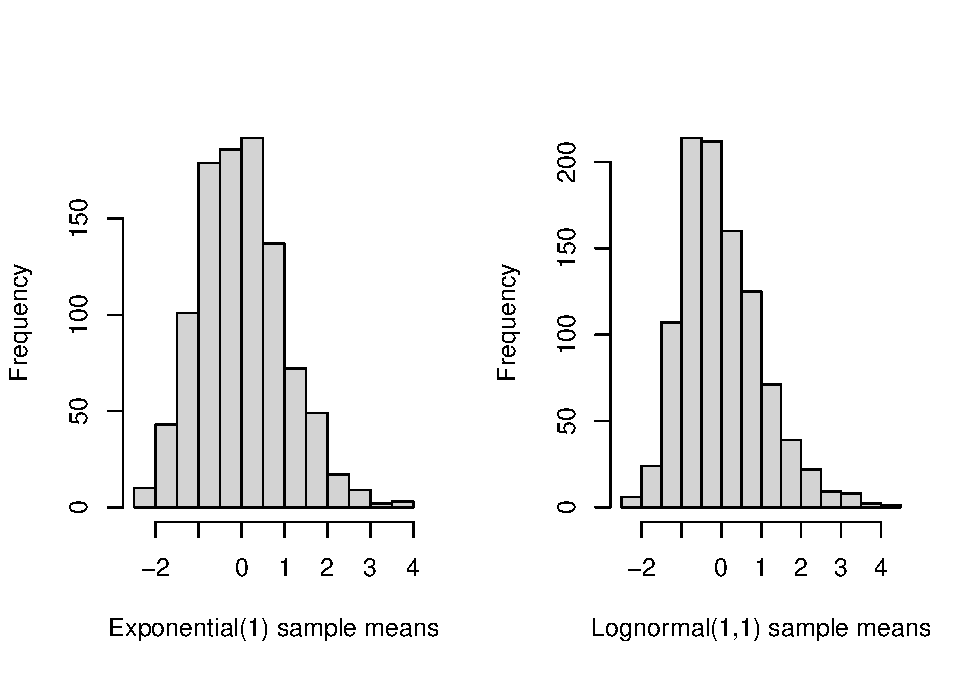
\includegraphics{10-Sampling-Distributions_files/figure-latex/unnamed-chunk-1-2.pdf}

As a final reminder, note the CLT does not apply to ``heavy-tailed'' distributions that lack a mean. For example, the Cauchy distribution is very likely to produce extreme values, and, as a result, it has no finite mean. Therefore, the CLT does not apply and it's unclear what will be the sampling distribution of it's sample mean. It turns out the sample mean is still Cauchy-distributed---taking the average of Cauchy samples does not reduce uncertainty at all. For an illustration, see the Monte-Carlo-approximated distribution of the sample mean of 50 samples from a Cauchy population:

\includegraphics{10-Sampling-Distributions_files/figure-latex/unnamed-chunk-2-1.pdf}

\hypertarget{sample-variance}{%
\section{Sample Variance}\label{sample-variance}}

Let \(X_1, X_2, \ldots, X_n\) denote a random sample from a Normal population with mean \(\mu\) and variance \(\sigma^2\). Denote the sample variance by \(S^2_n = \frac{1}{n-1}\sum_{i=1}^n (X_i - \overline X_n)^2\). Next, we will discover the sampling distribution of the (normal) sample variance.

First, we need to establish the fact that if \(Z\sim N(0,1)\), then \(Z^2\) has what is called a Chi-squared distribution, with one ``degree of freedom''---this is the parameter of this distribution. This Chi-squared distribution has MGF \(\left(1-2t\right)^{-k/2}\) where \(k\) is the degrees of freedom parameter. It's corresponding density function is
\[f(x) = 2^{-k/2}\left[\Gamma(k/2)\right]^{-1}x^{k/2-1}e^{-x/2},\quad x>0\]
and you might recognize this as a Gamma distribution with shape \(k/2\) and rate \(1/2\), so it's mean is \((k/2)/(1/2) = k\). Ww can establish this fact by the MGF technique. Evaluate the MGF of \(Z^2\) as follows:

\begin{align*}
M_{Z^2}(t) &= E(e^{tZ^2}) = \int_{-\infty}^{\infty} e^{tz^2}\frac{1}{\sqrt{2\pi}}e^{-\tfrac12 z^2}dz\\
& = \int_{-\infty}^{\infty} \frac{1}{\sqrt{2\pi}} e^{-\frac{1}{2\frac{1}{1-2t}}z^2}dz\\
& = \sqrt{\frac{1}{1-2t}}\int_{-\infty}^{\infty} \frac{1}{\sqrt{2\pi\frac{1}{1-2t}}} e^{-\frac{1}{2\frac{1}{1-2t}}z^2}dz\\
& = \sqrt{\frac{1}{1-2t}}
\end{align*}
where the last inequality follows from the fact the integrand is a normal density function with mean zero and variance \(\frac{1}{1-2t}\) (provided \(t<2\)) so that the integral equals one. This shows \(Z^2\) is Chi-squared distributed with \(1\) degree of freedom.

As we've many times, the MGF argument works particularly well with sums of independent random variables. If \(Z_1, Z_2, \ldots, Z_n\) are iid standard normal, then \(\sum_{i=1}^n Z_i^2\) is Chi-squared distributed with \(n\) degrees of freedom. To show this, simply show the MGF of \(\sum_{i=1}^n Z_i^2\) equals \(\left(1-2t\right)^{-n/2}\) using the previous result for \(n=1\), the definition of the MGF, and independence.

Next, we'll show a linear transformation of the the sample variance has a Chi-squared distribution with \(n-1\) degrees of freedom.

Start by making the linear transformation
\[\frac{(n-1)S_n^2}{\sigma^2} = \sum_{i=1}^n \left(\frac{X_i - \overline X_n}{\sigma}\right)^2.\]
Here's the main trick: add and subtract \(\mu\) inside the square in the sum, then expand the square and simplify:
\begin{align*}
\frac{(n-1)S_n^2}{\sigma^2} &= \sum_{i=1}^n \left(\frac{X_i - \mu + \mu - \overline X_n}{\sigma}\right)^2\\
& = \sum_{i=1}^n \left(\frac{X_i - \mu}{\sigma}\right)^2 + 2\sum_{i=1}^n \left(\frac{X_i - \mu}{\sigma}\right)\left(\frac{\mu - \overline X_n}{\sigma}\right) + \sum_{i=1}^n \left(\frac{\mu - \overline X_n}{\sigma}\right)^2\\
& = \sum_{i=1}^n \left(\frac{X_i - \mu}{\sigma}\right)^2 - 2n\left(\frac{\overline X_n - \mu}{\sigma}\right)^2 + n\left(\frac{\overline X_n - \mu}{\sigma}\right)^2\\
& = \sum_{i=1}^n \left(\frac{X_i - \mu}{\sigma}\right)^2 - n\left(\frac{\overline X_n - \mu}{\sigma}\right)^2\\
& = \sum_{i=1}^n \left(\frac{X_i - \mu}{\sigma}\right)^2 - \left(\frac{\overline X_n - \mu}{\sigma/\sqrt{n}}\right)^2
\end{align*}

So far, we have shown
\[\sum_{i=1}^n \left(\frac{X_i - \overline X_n}{\sigma}\right)^2 = \sum_{i=1}^n \left(\frac{X_i - \mu}{\sigma}\right)^2 - \left(\frac{\overline X_n - \mu}{\sigma/\sqrt{n}}\right)^2.\]

The first term on the right hand side is a summation of \(n\) squares of independent, standard normal r.v.'s \(Z_i = \frac{X_i - \overline X_n}{\sigma}\). Baed on our previous result, this sum must be distributed as Chi-squared with \(n\) degrees of freedom. The second term on the right is also the square of a standard normal random variable, so it must be distributed as Chi-squared with one degree of freedom. Consequently, the sum on the left hand side must be a Chi-squared random variable with \(n-1\) degrees of freedom.

\hypertarget{large-sample-sampling-distribution-of-sample-variance}{%
\subsection{Large-sample sampling distribution of sample variance}\label{large-sample-sampling-distribution-of-sample-variance}}

If \(X_1, X_2, \ldots, X_n\) is a random sample from a distribution with at least 4 finite moments, then the sample variance \(S_n^2\) is approximately normally distributed for large \(n\). To see this, note
\[S_n^2 = \frac{1}{n-1}\sum_{i=1}^n (X_i - \overline X_n)^2 \approx \frac{1}{n}\sum_{i=1}^n Z_i\]
where \(Z_i = (X_i - \mu)^2\). The latter expression is a sample average of iid random variables, and, as such, the CLT implies (the centered and scaled transformation of) it has a limiting normal distribution. This reasoning can be made rigorous.

\hypertarget{sampling-distribution-of-studentized-sample-mean}{%
\section{Sampling distribution of studentized sample mean}\label{sampling-distribution-of-studentized-sample-mean}}

Let \(X_1, X_2, \ldots, X_n\) be a random sample from a normal population with mean \(\mu\) and variance \(\sigma^2\); and, let \(\overline X_n\) and \(S_n^2\) denote the sample mean and sample variance, respectively.

Let
\[T_n:=\frac{\overline X_n - \mu}{\sqrt{S_n^2 / n}}\]
denote the ``studentized sample mean''. \(T_n\) is the standardized sample mean---\(\overline X_n\) minus \(\mu\) and divided by \(\sqrt{\sigma^2/n}\)---with the true variance replaced by its estimate, the sample variance.

The standardized sample mean has a standard normal distribution (even approximately so for non-normal random samples by the CLT), but the studentized sample mean is \emph{not} normally-distributed. Rather, the studentized sample mean has a Student's \(t\) distribution with \((n-1)\) degrees of freedom.

A Student's \(t\) random variable is defined in the following way: If \(Z\) is standard normal and independent of \$V \sim \(Chi-Squared\)(n-1)\$, then
\[T:=\frac{Z}{\sqrt{V/(n-1)}}\]
is a Student's \(t\) random variable with \(n-1\) degrees of freedom.

Rewriting the studentized sample mean, we have
\[T_n = \frac{\overline X_n - \mu}{\sqrt{S_n^2 / n}} = \frac{\frac{\overline X_n - \mu}{\sqrt{\sigma^2 / n}}}{\sqrt{(n-1)S_n^2/\{(n-1)\sigma^2\}}} = \frac{Z}{\sqrt{V/(n-1)}}.\]
It remains to verify \(\overline X_n\) and \(S_n^2\) are independent, and a sketch of this result is given next.

\hypertarget{part-of-students-theorem---indepndence-of-overline-x_n-and-s_n2}{%
\subsection{\texorpdfstring{Part of Student's Theorem - Indepndence of \(\overline X_n\) and \(S_n^2\)}{Part of Student's Theorem - Indepndence of \textbackslash overline X\_n and S\_n\^{}2}}\label{part-of-students-theorem---indepndence-of-overline-x_n-and-s_n2}}

Let \(Z_1, \ldots, Z_n\) be a random sample of standard normal random variables. Without loss of generality let's sketch a proof that \(\overline Z_n\) and \(W = \sum_{i=1}^n (Z_i - \overline Z_n)^2\) are independent. Define the matrix \(O_n\) to be the \(n\times n\) matrix with entries defined by:
\[For 1 \leq i \leq n-1, \quad o_{ij} = \Bigg\{ \begin{matrix} \frac{1}{\sqrt{i(i+1)}}, &j\leq i \\
-\frac{1}{\sqrt{i(i+1)}}, &j= i+1 
\end{matrix}\]
and zero otherwise; except that \(o_{nj} = n^{-1/2}\). Then, it can be checked that \(O_n\) is \emph{orthogonal}, i.e., \(O_n^\top O_n = I_n\), the identity. Next, define the vectors \(Z = (Z_1, \ldots, Z_n)^\top\) and \(Y = O_n Z\). By construction of \(O_n\) we have
\[Y^\top Y = Z^\top O_n^\top O_n Z = Z^\top Z = \sum_{i=1}^n Z_i^2.\]
And, we also have
\[Y_n = \sum_{i=1}^n \frac{Z_i}{\sqrt{n}} = \sqrt{n} \overline Z_n.\]
Therefore,
\[\sum_{i=1}^{n-1}Y_i^2 = \sum_{i=1}^{n}Y_i^2 - Y_n^2 = Z^\top Z - n\overline Z_n^2 = W.\]
So far, we have shown \(\overline Z_n\) is a function of \(Y_n\) and \(W\) is a function of \(Y_1, \ldots, Y_{n-1}\). But, \(Y = O_n Z\) is normally distributed with covariance \(O_n^\top O_n = I_n\). Therefore, \(Y_i\), \(i=1, \ldots, n\), are independent, which implies \(\overline Z_n\) and \(W\) are independent.

\hypertarget{differences-of-sample-means}{%
\section{Differences of Sample Means}\label{differences-of-sample-means}}

So far we have considered statistics baed on a single random sample. Now, we'll consider statistics based on separate random samples from two populations. First, consider a random sample \(X_1, X_2, \ldots, X_{n}\) from a normal distribution with mean and variance \(\mu_X\) and \(\sigma_X^2\) and another random sample \(Y_1, Y_2, \ldots, Y_m\) from a different normal distribution with mean and variance \(\mu_Y\) and \(\sigma_Y^2\).

\hypertarget{standarized-difference}{%
\subsection{Standarized difference}\label{standarized-difference}}

The standardized difference of means is given by
\[Z = \frac{\overline X_n - \overline Y_m - (\mu_X - \mu_Y)}{\sqrt{\frac{\sigma_X^2}{n} + \frac{\sigma_Y^2}{m}}}\]
and follows a standard normal distribution.

\hypertarget{studentized-difference-equal-variances}{%
\subsection{Studentized difference, equal variances}\label{studentized-difference-equal-variances}}

Suppose \(\sigma_X^2 = \sigma_Y^2\), and define the \emph{pooled sample variance} \(S_P^2 = \frac{(n-1)S_X^2 + (m-1)S_Y^2}{n+m-2}\). The studentized difference of sample means is defined by
\[T = \frac{\overline X_n - \overline Y_m - (\mu_X - \mu_Y)}{\sqrt{S_p^2(\frac{1}{n}+\frac{1}{m})}}\]
follows a Student's \(t\) distribution with \(n+m - 2\) degrees of freedom.

\hypertarget{studentized-difference-unequal-variances}{%
\subsection{Studentized difference, unequal variances}\label{studentized-difference-unequal-variances}}

When the population variances are unequal a different version of the studentized difference of means is sometimes used:
\[T = \frac{\overline X_n - \overline Y_m - (\mu_X - \mu_Y)}{\sqrt{\frac{S_X^2}{n}+\frac{S_Y^2}{m}}}.\]
This difference does not have an exact \(t\) distribution, but can be approximated well by a \(t\) distribution with degrees of freedom given by Satterthwaite's formula:
\[df = \frac{\left(\frac{S_X^2}{n}+\frac{S_Y^2}{m}\right)^2}{\frac{1}{n-1}\left(\frac{S_X^2}{n}\right)^2 + \frac{1}{m-1}\left(\frac{S_Y^2}{m}\right)^2}.\]
Since the degrees of freedom is an integer-valued parameter the result of this formula is \emph{rounded down} to the nearest integer.

\hypertarget{ratios-of-sample-variances}{%
\section{Ratios of Sample Variances}\label{ratios-of-sample-variances}}

As above, consider a random sample \(X_1, X_2, \ldots, X_{n}\) from a normal distribution with mean and variance \(\mu_X\) and \(\sigma_X^2\) and another random sample \(Y_1, Y_2, \ldots, Y_m\) from a different normal distribution with mean and variance \(\mu_Y\) and \(\sigma_Y^2\).

If \$U\sim \$Chi-Squared with df \(n-1\) and \$V\sim \$Chi-Squared with df \(m-1\) and \(U\) and \(V\) are independent, then
\[F := \frac{U/(n-1)}{V/(m-1)}\]
has an F distribution with two degrees of freedom parameters \(df1 = n-1\) and \(df2 = m-1\), often called the numerator and denominator degrees of freedom.

If \(S_X^2\) and \(S_Y^2\) are sample variances, then
\[\frac{\frac{(n-1)S_X^2}{\sigma_X^2(n-1)}}{\frac{(m-1)S_Y^2}{\sigma_Y^2(m-1)}} = \frac{S_X^2/\sigma_X^2}{S_Y^2/\sigma_Y^2}\]
has an \(F(n-1, m-1)\) distribution.

\hypertarget{statistical-estimation}{%
\chapter{Statistical Estimation}\label{statistical-estimation}}

\hypertarget{vocabulary}{%
\section{Vocabulary}\label{vocabulary}}

We consider experiments in which a random sample of observations is taken from a population. The sampling distribution of observations is known up to the value(s) of some \emph{population parameter(s)}. The goal of this chapter is to study \emph{estimation}---approximation of these unknown parameters by \emph{statistics}, functions of the sample data. An \emph{estimator} is the random variable version of a statistic and has a corresponding sampling distribution. By virtue of being called an estimator we assume this statistic is ``close'' to the true parameter value in some sense. An \emph{estimate} is a value of an estimator after the data is collected and the estimator computed; it is a fixed, non-random value.

For example, consider an experiment sampling \(n\) iid random samples from a Normal population with unknown mean \(\mu\) and variance \(1\). Here \(\mu\) is the parameter we wish to estimate. An intuitive estimator is the sample mean statistic \(\overline X_n = n^{-1}\sum_{i=1}^n X_i\). When the data is collected we refer to the calculated sample mean---the estimate of \(\mu\)---as lowercase \(\overline x_n\).

\hypertarget{properties-of-estimators}{%
\section{Properties of Estimators}\label{properties-of-estimators}}

It will become apparent that estimators are not unique---there are very often several seemingly reasonable estimators for a single parameter. Therefore we ought to be concerned with choosing the ``best'' estimator according to some criteria. Different criteria will lead to different ``best'' estimators.

\hypertarget{bias-and-unbiasedness}{%
\subsection{Bias and Unbiasedness}\label{bias-and-unbiasedness}}

Consider a generic parameter denoted \(\theta\) and imagine an estimator for \(\theta\) called \(\hat\theta_n\), which is a statistic and, hence, a random variable. We say \(\hat\theta_n\) is \emph{unbiased} if \(E(\hat\theta_n)=\theta\) where the expectation is taken with respect to the sampling distribution of \(\hat\theta_n\). For example, the sample mean \(\overline X_n\) is unbiased for the population mean \(\mu\) (so long as the population mean exists):
\begin{align*}
E(\overline X_n) &= E\left(n^{-1}\sum_{i=1}^n X_i\right)\\
& = n^{-1}\sum_{i=1}^n E(X_i)\\
& = n^{-1}\sum_{i=1}^n \mu\\
& = \mu.
\end{align*}
An unbiased estimator commits no systematic errors in estimating the parameter. In contrast, a biased estimator of a univariate real-valued parameter systematically underestimates or overestimates the parameter. Consider biased \(\hat\theta_n\) such that \(E(\hat\theta_n) = \theta + 1\). We \textbf{expect} \(\hat\theta_n\) to be 1 more than \(\theta\)---hence we expect it to overestimate.

\hypertarget{minimum-variance-unbiased-estimators}{%
\subsection{Minimum Variance Unbiased Estimators}\label{minimum-variance-unbiased-estimators}}

Besides a finite mean, estimators often have a finite variance. And, intuitively, we would tend to prefer an estimator with low variance to one with high variance, particularly if both are unbiased. If we insist on an unbiased estimator, then the ``best'' unbiased estimator is the unbiased estimator with smallest variance among all unbiased estimators.

It is not obvious how one would find the lowest variance estimator among all unbiased estimators. One result, due to CR Rao and Harald Cramer, provides a lower bound on the variance of an unbiased estimator. This lower bound can be checked by computing the variance of a given unbiased estimator, and, if they match, this implies the given estimator is the MVUE. We describe this procedure below.

Let \(f(x;\theta)\) denote the density of the data and let \(\theta\) denote a univariate parameter. Let \(\ell(x;\theta) := \log(f(x;\theta))\), the natural logarithm of the density. Define the \emph{Fisher Information} for one data point by
\[I(\theta) = E\left[\left(\frac{\partial \ell(x;\theta)}{\partial\theta}\right)^2\right].\]
The Fisher information for a random sample of size \(n\) is \(n\) times \(I(\theta)\). Then, Cramer and Rao showed that if \(\hat\theta_n\) is unbiased, its variance cannot be smaller than
\[V(\hat\theta_n)\geq \left[nI(\theta)\right]^{-1}\]
where \(\theta\) is the true parameter value.

Example: Let \(X_1, \ldots, X_n\) be a random sample from a normal population with variance 1 and mean \(\mu\) and consider the estimator \(\overline X_n\). The logarithm of the density function is
\[\ell(f(x;\mu)) = -\log(\sqrt{2\pi}) - \tfrac12(x - \mu)^2\]
with \(\mu-\)derivative \(x - \mu\). Therefore, the Fisher Information is
\[I(\mu) = E[(X - \mu)^2] = 1\]
since it is, by definition, equal to the variance. The Cramer-Rao lower bound is
\[V(\hat\theta_n)\geq \frac{1}{n},\]
and we know \(V(\overline X_n) = 1/n\) so the sample mean \(\overline X_n\) is, indeed, the MVUE for this experiment.

\hypertarget{mean-squared-error-and-bias-variance-tradeoff}{%
\subsection{Mean Squared Error and Bias-Variance tradeoff}\label{mean-squared-error-and-bias-variance-tradeoff}}

As described above a common strategy is to select an unbiased estimator, preferably one with low (or the lowest) variance. On the other hand, one may prefer a biased estimator over an unbiased one if the bias is low and there is substantial reduction in variance. One way to choose estimators that balance bias and variance is to consider their mean squared error (MSE), defined by
\[MSE(\hat\theta_n) = E[(\hat\theta_n - \theta)^2] = Bias(\theta_n)^2 + V(\hat\theta_n).\]
It is left as an exercise to the reader to show the MSE equals the sum of estimator variance and squared bias. For the above reasons the estimator minimizing the MSE may be preferable even to the MVUE.

Example: Estimation of a normal population variance
The usual variance estimator is the sample variance \(S^2_n = \frac{1}{n-1}\sum_{i=1}^n (X_i - \overline X_n)^2\). It can be checked this estimator is unbiased. And, it is a bit of a pain, but it can be shown that \(V(S_n^2) = \frac{2\sigma^4}{n-1}\). Now, consider an alternative estimator that is a constant multiple of \(S^2_n\), say \(c S_n^2\) for some \(c>0\). The MSE of this estimator is
\begin{align*}
MSE(cS_n^2) &= V(cS_n^2) + Bias(cS_n^2)^2\\
& = c^2\frac{2\sigma^4}{n-1} + [E(cS_n^2) - \sigma^2]^2\\
& = c^2\frac{2\sigma^4}{n-1} + (c\sigma^2 - \sigma^2)^2\\
& = c^2\frac{2\sigma^4}{n-1} + \sigma^4(c-1)^2.
\end{align*}
Differentiate w.r.t. \(c\) to find
\[\frac{\partial MSE}{\partial c} = 2c \frac{2\sigma^4}{n-1} + 2(c-1)\sigma^4.\]
Set this equal to zero and solve for \(c\). We get
\[c = \frac{2\sigma^4}{\frac{4\sigma^4}{n-1} + 2\sigma^4} = \frac{n-1}{2+n-1} = \frac{n-1}{n+1}.\]
This means the minimim MSE estimator (at least among those that are multiples of \(S_n^2\)) is actually \(\frac{1}{n+1}\sum_{i=1}^n (X_i - \overline X_n)^2\).

\hypertarget{consistency}{%
\subsection{Consistency}\label{consistency}}

Besides avoiding systematic estimation errors and having low variance, we would expect that as more and more data is collected an estimator should get better and better---and get ``closer'' to the true parameter, in some sense. This intuition is captured mathematically by \emph{consistency}. An estimator is consistent if for any \(c>0\), however small,
\[\lim_{n\rightarrow \infty} P(|\hat\theta_n-\theta|>c) = 0.\]
Dissecting this definition from the inside out we first note \(|\hat\theta_n - \theta|\) is the random estimation error. Then, \(|\hat\theta_n-\theta|>c\) says the error is at least \(c\). Since the error is a random variable we attach a probability to the chance the error is at least \(c\), which is \(P(|\hat\theta_n-\theta|>c)\). And, consistency says this probability must vanish as we accumulate data. So, the chance of an error of any size \(c\) or bigger vanishes. Taking complements, this is equivalent to saying
\[\lim_{n\rightarrow \infty} P(|\hat\theta_n-\theta|<c) = 1,\]
which means \(\hat\theta_n\) is within \(c\) of \(\theta\) with probability going to 1.

One way to show an estimator is consistent is to show it is unbiased and has variance that vanishes as \(n\rightarrow 0\). One example is the sample mean, which is unbiased and has variance \(\sigma^2/n\). Then, consistency follows by Chebyshev's inequality, which says: for any r.v. \(X\) with finite mean and variance \((\mu, \sigma^2)\),
\[P(|X - \mu|>c)\leq \frac{\sigma^2}{c^2}\]
for any \(c>0\). In the context of estimation, we have
\[P(|\hat\theta_n - E(\hat\theta_n)|>c) \leq \frac{Var(\hat\theta_n)}{c^2}.\]
Now, suppose \(\hat\theta_n\) is unbiased and its variance vanishes in \(n\). Then, the above statement says
\[P(|\hat\theta_n - \theta|>c) \leq s_n.\]
for a sequence \(s_n\) satisfying \(\lim_{n\rightarrow \infty} s_n = 0\). Checking the definition we see this means \(\hat\theta_n\) is consistent. A similar argument can work for biased estimators as well, provided the bias also vanishes as \(n\rightarrow\infty\). Such estimators are called \emph{asymptotically unbiased}. One such example is the minimum MSE estimator of \(\sigma^2\) from the previous section. It has bias \(\sigma^2(\frac{n-1}{n+1}-1)\) which has limit zero.

\hypertarget{finding-estimators---method-of-moments}{%
\section{Finding estimators - Method of Moments}\label{finding-estimators---method-of-moments}}

So far we've discussed desirable properties of estimators but not where these estimators come from. How do we find estimators in the first place? One strategy is based on the fact population parameters often are related to population moments. Then, we can find estimators by replacing population moments by sample moments and referring back to the relationship between the moments and parameters. The simplest example of the method of moments is estimation of the population mean by the sample mean.

Example: Suppose a population is modeled as a Gamma distribution with shape and rate parameters \((\alpha, \beta)\). The population mean is \(\alpha / \beta\) and the population variance is \(\alpha / \beta^2\). This means the population second raw moment is \(\alpha / \beta^2 + (\alpha / \beta)^2\). We can estimate \((\alpha, \beta)\) by matching the sample and population raw moments as follows:
\begin{align*}
n^{-1}\sum_{i=1}^n X_i &= \alpha/\beta^2\\
n^{-1}\sum_{i=1}^n X_i^2 &= \alpha/\beta^2 + (\alpha / \beta)^2.
\end{align*}
Solving the system by substitution we have
\begin{align*}
\hat\alpha = \frac{\hat\mu_2' - \hat\mu_1'}{\hat\mu_1'}\\
\hat \beta = \sqrt{\frac{\hat\mu_2' - \hat\mu_1'}{(\hat\mu_1')^2}},
\end{align*}
where \(\hat\mu_1'\) and \(\hat\mu_2'\) indicate the 1st and second raw sample moments \(n^{-1}\sum_{i=1}^n X_i\) and \(n^{-1}\sum_{i=1}^n X_i^2\).

Example: Suppose we will take a random sample of size \(n\) from a continuous uniform distribution supported on the interval \((a,b)\) where the endpoints are unknown. We know that \(E(X) = \frac{a+b}{2}\) and \(V(X) = \frac{(b-a)^2}{12}\) so that \(E(X^2) = \frac{(b-a)^2}{12} + \frac{(a+b)^2}{4}\). Then, we find estimators for \((a,b)\) by solving
\begin{align*}
n^{-1}\sum_{i=1}^n X_i &= \frac{a+b}{2}\\
n^{-1}\sum_{i=1}^n X_i^2 &= \frac{(b-a)^2}{12} + \frac{(a+b)^2}{4}.
\end{align*}
With some work, you should find \((\hat a, \hat b) = (\hat\mu_1' - \sqrt{3\hat\mu_2'}, \, \hat\mu_1'+\sqrt{3\hat\mu_2'})\). That's not so intuitive\ldots{} What about using the sample minimum and maximum\ldots{}

\hypertarget{method-of-maximum-likelihood}{%
\section{Method of Maximum Likelihood}\label{method-of-maximum-likelihood}}

Again consider a random sample \(X_1, \ldots, X_n\) from a population synonymous with a density function \(f(x;\theta)\) for an unknown parameter \(\theta\). For the time being consider only scalar \(\theta\). The \emph{likelihood function} is the joint PDF of the data viewed as a function of the parameter, and may be treated either as a random function or as a deterministic function depending on whether the data are treates as random variables or as observed values, so pay close attention to the context. For iid data the likelihood can be written
\[L(\theta;X_1, \ldots, X_n) = \prod_{i=1}^n f(X_i;\theta).\]

For the purpose of estimating \(\theta\) we view the likelihood as a deterministic function given observations. Then, it acts as a sort of ``ranking function'' that provides a quantitative comparison of how well different parameter values agree with the observed data. The idea is to select as an estimate the parameter value that maximizes the likelihood/agreement with the data. To explain this concept of agreement with the data a bit more suppose the data come from a discrete population so that \(f(x;\theta)\) is a PMF rather than a density---this makes the interpretation easier. Then \(\prod_{i=1}^n f(X_i;\theta)\) is a the probability of observing the data for a given parameter value \(\theta\). Choosing \(\theta\) to maximize this probability means selecting the distribution that gives the highest probability assignment to the data that was actually observed.

Example: Suppose our random sample comes from an Exponential distribution with rate \(\lambda\). The likelihood function equals
\begin{align*}
L(\lambda, x_1, \ldots, x_n) &= \prod_{i=1}^n \lambda^{-1}e^{-x_i/\lambda}\\
& = \lambda ^{-n}e^{-\tfrac1\lambda\sum_{i=1}^n x_i}.
\end{align*}

Take the first derivative of the likleihood with respect to \(\lambda\):
\[\frac{\partial L}{\partial \lambda} = -n\lambda^{-(n+1)}e^{-\tfrac1\lambda \sum_{i=1}^n x_i} + \lambda^{-n}e^{-\tfrac1\lambda\sum_{i=1}^n x_i}\left(\lambda^{-2}\sum_{i=1}^n x_i\right)\]
Set \(\tfrac{\partial L}{\partial \lambda}\) equal to zero and solve for \(\lambda\) to obtain the MLE:
\begin{align*}
\frac{\partial L}{\partial \lambda} = 0 & \Rightarrow -n\lambda^{-1} + \tfrac{1}{\lambda^2}\sum_{i=1}^n x_i = 0\\
& \Rightarrow n\lambda = \sum_{i=1}^n x_i\\
& \Rightarrow \hat{\theta}_{MLE} = \overline x_n.
\end{align*}

Example: Suppose our random sample comes from a Uniform distribution on the interval \((0,\theta)\). The likelihood function equals
\begin{align*}
L(\lambda, x_1, \ldots, x_n) &= \prod_{i=1}^n \frac{1}{\theta}1(0\leq x_i\leq \theta) \\
& = \theta^{-n}\prod_{i=1}^n 1(0\leq x_i\leq \theta).
\end{align*}

We cannot simply maximize this likelihood function by taking the first derivative because the indicator functions are not everywhere differentiable w.r.t. \(\theta\). Instead, note that the function \(\theta^{-n}\) is monotonically decreasing in \(\theta\); so, this function prefers small \(\theta\). On the other hand, the function \(\prod_{i=1}^n 1(0\leq x_i\leq \theta)\) is constant and equal to 1 so long as \(\theta \geq \max_{i=1, \ldots, n} x_i\); otherwise, this function is zero and so is the likelihood (and the likelihood cannot be less than zero!). This means we should choose \(\theta = \max_{i=1, \ldots, n} x_i\) to maximize the likelihood. Therefore, the MLE of \(\theta\) is \(\hat\theta_{MLE} = max_{i=1, \ldots, n} x_i\).

Multivariate Example: Consider estimation of both the mean and variance parameters of a normal population based on a random sample of size \(n\) denoted \(X^n = (X_1, \ldots, X_n)^\top\). The likelihood is a function of two parameters \((\mu, \sigma^2)\):
\[L(\mu, \sigma^2;X^n) = (2\pi\sigma^2)^{-n/2}\exp\left(-\frac{1}{2\sigma^2}\sum_{i=1}^n (X_i-\mu)^2\right).\]
The loglikelihood is easier to maximize so take the log and find
\[\ell(\mu, \sigma^2;X^n) = -\frac{n}{2}\log (2\pi\sigma^2) -\frac{1}{2\sigma^2}\sum_{i=1}^n (X_i-\mu)^2. \]
To find the MLEs we need to compute the gradient vector:
\begin{align*}
\frac{\partial\ell}{\partial \mu} &= \frac{1}{\sigma^2}\sum_{i=1}^n (X_i-\mu)\\
\frac{\partial\ell}{\partial \sigma^2} &= -\frac{n}{2\sigma^2} + \frac{1}{2\sigma^4}\sum_{i=1}^n (X_i-\mu)^2.
\end{align*}
Setting \(\frac{\partial\ell}{\partial \mu}=0\) we immediately find \(\hat\mu_{MLE} = \overline X_n\). Substituting this estimate for \(\mu\) in the second equation we find \(\hat\sigma^2_{MLE} = \frac{1}{n}\sum_{i=1}^n (X_i-\overline X_n)^2\), the version of the sample variance with denominator \(n\) instead of \(n-1\). The following result says the MLE has variance approximately equal to the reciprocal of the Fisher information when the parameter is a scalar. In the multivariate setting the analogous quantity is the inverse Fisher information matrix, which is the inverse of the expectation of \(-1\) times the matrix of second partial derivatives of the loglikelihood. Let's calculate this variance-covariance matrix next. First, we need to compute the matrix of second partial derivatives of the loglikelihood:\\
\begin{align*}
\frac{\partial^2\ell}{\partial \mu^2} &= -\frac{n}{\sigma^2}\\
\frac{\partial^2\ell}{\partial \mu\partial\sigma^2} &= -\frac{1}{\sigma^4}\sum_{i=1}^n (X_i-\mu)\\
\frac{\partial^2\ell}{\partial (\sigma^2)^2} &= \frac{n}{2\sigma^4} - \frac{1}{\sigma^6}\sum_{i=1}^n (X_i-\mu)^2
\end{align*}
Next, take the expectation of these partial derivatives and multiply by \(-1\):
\begin{align*}
-E(\frac{\partial^2\ell}{\partial \mu^2}) &= \frac{n}{\sigma^2}\\
-E(\frac{\partial^2\ell}{\partial \mu\partial\sigma^2}) &= 0\\
-E(\frac{\partial^2\ell}{\partial (\sigma^2)^2}) &= -\frac{n}{2\sigma^4} + \frac{n}{\sigma^4} = \frac{n}{2\sigma^4}.
\end{align*}
Finally, find the inverse of the matrix:
\[\begin{bmatrix}
\frac{n}{\sigma^2} &0 \\
0 &\frac{n}{2\sigma^4}.
\end{bmatrix}\]
Since this is a diagonal matrix, the inverse is simply the matrix of reciprocal values on the diagonal:
\[Cov(\hat\mu_{MLE}, \hat\sigma^2_{MLE}) \approx \begin{bmatrix}
\frac{\sigma^2}{n} &0 \\
0 &\frac{2\sigma^4}{n}.
\end{bmatrix}\]
according to the asymptotic results on MLEs given below. Since the unknown parameter \(\sigma^2\) shows up in this covariance matrix, in practice we replace it with its estimate, yielding the estimated covariance matrix
\[\widehat {Cov}(\hat\mu_{MLE}, \hat\sigma^2_{MLE}) \approx \begin{bmatrix}
\frac{\hat\sigma_{MLE}^2}{n} &0 \\
0 &\frac{2\hat\sigma_{MLE}^4}{n}.
\end{bmatrix}\]

\hypertarget{properties-of-mles}{%
\section{Properties of MLEs}\label{properties-of-mles}}

Maximum likelihood estimation is a powerful technique because it produces estimators with good properties in a wide range of settings. These properties include consistency, asymptotic unbiasedness, asymptotic efficiency (attainment of the Cramer-Rao lower variance bound), and asymptotic normality; subject to the fulfilment of ``regularity conditions''. These conditions include
1. Indentifiability - the CDF \(F(x; \theta)\) satisfies \(\theta\ne\theta\Rightarrow F(x;\theta)\ne F(x;\theta')\) for all \(x\)
2. The sample sapce of the PDF does not depend on \(\theta\).
3. The true \(\theta^\star\) is not on the boundary of the domain of \(\theta\).
4. The PDF \(f(x;\theta)\) is three-times differentiable in \(\theta\), and for all \(\theta\) in a neighborhood of \(\theta^\star\) the function \(|\frac{\partial^3}{\partial\theta^3}\log f(X;\theta)|\) is bounded by a function \(M(X)\) with finite mean.
5. We can differentiate \(\int f(x;\theta)dx\) twice wr.t. \(\theta\) by exchanging the order of integration and differentiation (limits).

Some of these conditions can be weakened, depending on the property one is trying to prove, and in some cases by making more advanced arguments, but these are the conditions we will use to establish asymptotic normality below.

Proof sketch of asymptotic normality:

Define the loglikelihood function \(\ell(\theta):=\log L(\theta;X_1, \ldots, X_n)\) and expand its first derivative in Taylor series about the MLE \(\hat\theta_n\) as follows:
\[\ell'(\hat\theta_n) = \ell'(\theta^\star) + (\hat\theta_n - \theta^\star)\ell''(\theta^\star) + \tfrac12(\hat\theta_n - \theta^\star)^2\ell'''(\tilde\theta),\]
where \(\tilde\theta\) is some value between \(\hat\theta_n\) and \(\theta^\star\) by Taylor's theorem. Rearranging terms we have
\[\sqrt{n}(\hat\theta_n - \theta^\star) = \frac{n^{-1/2}\ell'(\theta^\star)}{-n^{-1}\ell''(\theta^\star) - (2n)^{-1}(\hat\theta_n-\theta^\star)\ell'''(\tilde\theta)}.\]
The CLT implies the numerator on the RHS above converges in distribution to \(N(0, I(\theta^\star))\). The weak LLN implies the first term in the denominator converges to \(I(\theta^\star)\) in probability. By the fourth regularity condition and the weak LLN the term \(\tfrac1n \ell'''(\tilde\theta)\) in the denominator converges to \(E(M(X))\) and hence, is \emph{bounded in probability}. This term is multiplied by \((\hat\theta_n - \theta^\star)\) which converges to zero by consistency, and hence this last product term in the denominator converges to zero in probability. Together, these bounds imply
\[\sqrt{n}(\hat\theta_n - \theta^\star)\rightarrow N(0,I(\theta^\star)^{-1}).\]
The formal support for this last claim is provided by Slutsky's Theorem which we'll not cover here. We also used consistency in this proof sketch which we haven't shown. This latter result provides the additional and stronger properties of asymptotic unbiasedness, efficiency, and normality.

  \bibliography{book.bib,packages.bib}

\end{document}
